%% ----------------------------------------
%%
%% NYU PhD thesis template.
%% Created by José Koiller 2007--2008.
%% Modified by Siddharth Krishna, 2019.
%%
%% ----------------------------------------


%% Use the first of the following lines during production to
%% easily spot "overfull boxes" in the output. Use the second
%% line for the final version.
%\documentclass[12pt,draft,letterpaper]{report}
\documentclass[12pt,oneside,letterpaper]{report}


% ----------------------------------------
% Macro to switch between draft version and final version
% ----------------------------------------

% Use or comment this to enable/disable draft version
% \def\draftversion{}
\newcommand{\draftfinal}[2]{\ifdefined\draftversion#1\else#2\fi}
\newcommand{\draftonly}[1]{\draftfinal{#1}{}}
\newcommand{\finalonly}[1]{\draftfinal{}{#1}}


% ----------------------------------------
% Thesis metadata
% ----------------------------------------

%% Replace the title, name, advisor name, graduation date and dedication below
%% with your own. Graduation months must be January, May or September.
\newcommand{\thesistitle}{A Mean-Field Optimal Control Formulation of GANs}
\newcommand{\thesisauthor}{Yirong Bian}
\newcommand{\thesisadvisor}{Professor Mathieu Laurière}
\newcommand{\thesisdept}{Mathematics}
\newcommand{\gradmonth}{May}
\newcommand{\gradyear}{2022}



% ----------------------------------------
% Layout and formatting
% ----------------------------------------

% Uncomment to get a big black box to spot "overfull hboxes"
\setlength{\overfullrule}{5pt}


%% Page layout (customized to letter paper and NYU requirements):
\RequirePackage[margin=1in, includefoot, letterpaper]{geometry}


%% Color definitions:
\RequirePackage[prologue]{xcolor}
\definecolor[named]{ThesisBlue}{cmyk}{1,0.1,0,0.1}
\definecolor[named]{ThesisYellow}{cmyk}{0,0.16,1,0}
\definecolor[named]{ThesisOrange}{cmyk}{0,0.42,1,0.01}
\definecolor[named]{ThesisRed}{cmyk}{0,0.90,0.86,0}
\definecolor[named]{ThesisLightBlue}{cmyk}{0.49,0.01,0,0}
\definecolor[named]{ThesisGreen}{cmyk}{0.20,0,1,0.19}
\definecolor[named]{ThesisPurple}{cmyk}{0.55,1,0,0.15}
\definecolor[named]{ThesisDarkBlue}{cmyk}{1,0.58,0,0.21}

% School color found from university's graphic identity site:
% http://www.nyu.edu/employees/resources-and-services/media-and-communications/styleguide.html
\definecolor{SchoolColor}{rgb}{0.3412, 0.0235, 0.5490} % purple
\definecolor{chaptergrey}{rgb}{0.2600, 0.0200, 0.4600} % dialed back a little
\definecolor{midgrey}{rgb}{0.4, 0.4, 0.4}

\usepackage{hyperref}
\hypersetup{colorlinks,
  linkcolor=ThesisDarkBlue,
  citecolor=ThesisPurple,
  urlcolor=ThesisDarkBlue,
  filecolor=ThesisDarkBlue}


%% Captions of Figures, tables
\RequirePackage[labelfont={bf,sf,small,singlespacing},
                textfont={sf,small,singlespacing},
                % justification={justified,RaggedRight},
                % singlelinecheck=false,
                margin=0pt,
                figurewithin=chapter,
                tablewithin=chapter]{caption}

%% Chapter headings, captions
\usepackage{fix-cm}
\RequirePackage[raggedright,sc]{titlesec}
\definecolor{gray75}{gray}{0.75}
\newcommand{\hsp}{\hspace{20pt}}

\titleformat{\chapter}[hang]
{\Huge\sc}
{\textcolor{SchoolColor}{\thechapter}\hsp\textcolor{gray75}{|}\hsp}
{0pt}{\Huge\sc\raggedright}
% [\textcolor{gray75}{|}\hsp\textcolor{SchoolColor}{\thechapter}]


%% The following makes chapters and sections, but not subsections,
%% appear in the TOC (table of contents). Increase to 2 or 3 to
%% make subsections or subsubsections appear, respectively. It seems
%% to be usual to use the "1" setting, however.
\setcounter{tocdepth}{2}

%% Sectional units up to subsubsections are numbered. To number
%% subsections, but not subsubsections, decrease this counter to 2.
\setcounter{secnumdepth}{2}

%% Use the following commands, if desired, during production.
%% Comment them out for final version.
%\usepackage{layout} % defines the \layout command, see below
%\setlength{\hoffset}{-.75in} % creates a large right margin for notes and \showlabels

%% Controls spacing between lines (\doublespacing, \onehalfspacing, etc.):
\usepackage{setspace}

%% Use the line below for official NYU version, which requires
%% double line spacing. For all other uses, this is unnecessary,
%% so the line can be commented out.
\finalonly{
  \doublespacing % requires package setspace, invoked above
}

%% For generating sample text.
%% Can be removed when you've replaced all \lipsum commands with your text.
\usepackage{lipsum}


% ----------------------------------------
% Comments and TODOs:
% ----------------------------------------

% Uncomment this to remove all comments
\newcommand{\nocomments}{}

% Uncomment this to remove all TODOs
\newcommand{\notodos}{}

% Comments and TODOs
\newcommand{\fcomment}[2]{\ifdefined\nocomments{}\else\footnote{\textcolor{red}{#1:} #2}\fi}
\newcommand{\todo}[1]{\ifdefined\notodos{}\else\textcolor{red}{TODO\ifstrempty{#1}{}{: #1}}\fi}
\newcommand{\ftodo}[1]{\ifdefined\notodos{}\else\fcomment{TODO}{#1}\fi}

% Author comments:
\newcommand{\aen}[1]{\fcomment{Emmy}{#1}}


% ----------------------------------------
% User-specific packages and macros
% ----------------------------------------

%% This inputs your auxiliary file with \usepackage's and \newcommand's:
%% It is assumed that that file is called "defs.tex".
% ----------------------------------------
% Packages
% ----------------------------------------

% 
% Place here your \usepackage's. Some recommended packages are already included.
%

% Graphics:
\usepackage[final]{graphicx}
%\usepackage{graphicx} % use this line instead of the above to suppress graphics in draft copies
%\usepackage{graphpap} % \defines the \graphpaper command

% Uncomment this to indent first line of each section:
% \usepackage{indentfirst}

% Good AMS stuff:
\usepackage{amsthm} % facilities for theorem-like environments
\usepackage[tbtags]{amsmath} % a lot of good stuff!

% Fonts and symbols:
\usepackage{amsfonts}
\usepackage{amssymb}

% Set the fonts
\RequirePackage[T1]{fontenc}
\ifxetex
  \RequirePackage[tt=false]{libertine}
\else
  \RequirePackage[tt=false, type1=true]{libertine}
\fi
\RequirePackage[varqu]{zi4}
\RequirePackage[libertine]{newtxmath}


% For typesetting inference rules
\usepackage{mathpartir}
% \usepackage{pftools}  % A local package
\newcommand{\bmmax}{2}
\usepackage{bm}

% Formatting tools:
%\usepackage{relsize} % relative font size selection, provides commands \textsmalle, \textlarger
%\usepackage{xspace} % gentle spacing in macros, such as \newcommand{\acims}{\textsc{acim}s\xspace}

% Page formatting utility:
%\usepackage{geometry}

\usepackage{booktabs}   %% For formal tables:
                        %% http://ctan.org/pkg/booktabs
\usepackage[labelformat=simple]{subcaption} %% For complex figures with subfigures/subcaptions
                        %% http://ctan.org/pkg/subcaption
% Options to subcaption are to label and refer to subfigures as Fig 1(a) etc.
\renewcommand\thesubfigure{(\alph{subfigure})}

\usepackage[T1]{fontenc} % needed for scaling fancy fonts (?)
\usepackage[utf8]{inputenc} % not sure this is needed

\usepackage{amssymb}
%\usepackage[table]{xcolor}


% For code
\usepackage[final]{listings}
\lstset{mathescape=true}

% For code highlighting
% \usepackage{bold-extra}

% Tikz
\usepackage{tikz}
\usetikzlibrary{matrix,arrows,positioning,calc,fit,backgrounds}

% To control enum item labelling/numbering
\usepackage[shortlabels, inline]{enumitem}
% To give custom item labels and reference them
\makeatletter
\newcommand{\myitem}[1][]{
  \protected@edef\@currentlabel{#1}%
\item[#1]
}
\makeatother

% To stop aligned env swallowing up []s
\usepackage{mathtools}

% To use ifstrempty
\usepackage{etoolbox}

% For math mode tables
\usepackage{array}
% A text column in array
\newcolumntype{L}{>$l<$}

% For \llbracket and \rrbracket
\usepackage{stmaryrd}

% For dashed boxes
\usepackage{dashbox}

% For big separating conjunction
\usepackage{scalerel}

% For mathpar environment
\usepackage{mathpartir}

\usepackage{xspace}
\usepackage{multirow}

% To stop citations overflowing lines
\usepackage{breakcites}

% For citet command
\usepackage{natbib}
\setcitestyle{%
    authoryear,%
    open={[},close={]},citesep={;},%
    aysep={},yysep={,},%
    notesep={, }}
\let\cite\citep

%%
%% Place here your \newtheorem's:
%%

\theoremstyle{plain}
\newtheorem{theorem}{Theorem}[chapter]
\newtheorem{conjecture}[theorem]{Conjecture}
\newtheorem{proposition}[theorem]{Proposition}
\newtheorem{lemma}[theorem]{Lemma}
\newtheorem{corollary}[theorem]{Corollary}
\theoremstyle{definition}
\newtheorem{example}[theorem]{Example}
\newtheorem{definition}[theorem]{Definition}
\theoremstyle{plain}


% ----------------------------------------
% Generic definitions
% ----------------------------------------
% Required packages: listings, tikz

% A footnote without a marker
\newcommand\blfootnote[1]{%
  \begingroup
  \renewcommand\thefootnote{}\footnote{#1}%
  \addtocounter{footnote}{-1}%
  \endgroup
}

\renewcommand{\le}{\leqslant}
\renewcommand{\ge}{\geqslant}
% \renewcommand{\emptyset}{\ensuremath{\varnothing}}
% \newcommand{\ds}{\displaystyle}

% Math stuff
\newcommand{\R}{\ensuremath{\mathbb{R}}}
\newcommand{\Q}{\ensuremath{\mathbb{Q}}}
\newcommand{\Z}{\ensuremath{\mathbb{Z}}}
\newcommand{\N}{\ensuremath{\mathbb{N}}}
\newcommand{\T}{\ensuremath{\mathbb{T}}}
\newcommand{\C}{\ensuremath{\mathbb{C}}}
\newcommand{\eps}{\varepsilon}
\newcommand{\closure}[1]{\ensuremath{\overline{#1}}}
%\newcommand{\acim}{\textsc{acim}\xspace}
%\newcommand{\acims}{\textsc{acim}s\xspace}
\newcommand{\Dense}{\textit{Dense}}



\newcommand{\Land}{\bigwedge}
\newcommand{\Lor}{\bigvee}
\newcommand{\es}{\emptyset}
\newcommand{\incl}{\subseteq}
\newcommand{\impl}{\Rightarrow}
\renewcommand{\iff}{\Leftrightarrow}
\newcommand{\ra}{\rightarrow}
\newcommand{\sat}{\vDash}
\newcommand{\notsat}{\nvDash}
\newcommand{\proves}{\vdash}
\newcommand{\provesIff}{\mathrel{\dashv\vdash}}
\newcommand{\boolTrue}{\top}
\newcommand{\boolFalse}{\bot}

\newcommand{\dom}{\operatorname{\mathsf{dom}}}
\newcommand{\range}{\operatorname{\mathsf{rng}}}
\newcommand{\restrict}[2]{{#1}|_{#2}}
\newcommand{\pto}{\rightharpoonup}

\newcommand{\defeq}{\coloneqq}
\newcommand{\defiff}{\vcentcolon\iff}

\newcommand{\pipe}{\triangleright}

%% Caligraphic
\newcommand{\Aa}{{\mathcal{A}}}
\newcommand{\Bb}{{\mathcal{B}}}
\newcommand{\Cc}{{\mathcal{C}}}
\newcommand{\Dd}{{\mathcal{D}}}
\newcommand{\Ee}{{\mathcal{E}}}
\newcommand{\Ff}{{\mathcal{F}}}
\newcommand{\Gg}{{\mathcal{G}}}
\newcommand{\Hh}{{\mathcal{H}}}
\newcommand{\Ii}{{\mathcal{I}}}
\newcommand{\Jj}{{\mathcal{J}}}
\newcommand{\Kk}{{\mathcal{K}}}
\newcommand{\Ll}{{\mathcal{L}}}
\newcommand{\Mm}{{\mathcal{M}}}
\newcommand{\Nn}{{\mathcal{N}}}
\newcommand{\Oo}{{\mathcal{O}}}
\newcommand{\Pp}{{\mathcal{P}}}
\newcommand{\Qq}{{\mathcal{Q}}}
\newcommand{\Rr}{{\mathcal{R}}}
\newcommand{\Ss}{{\mathcal{S}}}
\newcommand{\Tt}{{\mathcal{T}}}
\newcommand{\Uu}{{\mathcal{U}}}
\newcommand{\Vv}{{\mathcal{V}}}
\newcommand{\Ww}{{\mathcal{W}}}
\newcommand{\Yy}{{\mathcal{Y}}}
\newcommand{\Zz}{{\mathcal{Z}}}

% Wrappers: Parens, brackets, etc
% \newcommand{\op}[1]{\operatorname{#1}}
\newcommand{\paren} [1] {\ensuremath{ \left( {#1} \right) }}
\newcommand{\bigparen} [1] {\ensuremath{ \Big( {#1} \Big) }}
% \newcommand{\bracket}[1]{\left[#1\right]}
\newcommand{\tuple}[1]{\ensuremath{\langle #1 \rangle}}
\newcommand{\abs}[1]{\ensuremath{\lvert #1 \rvert}}
% \newcommand{\set}[1]{\ensuremath{\left\{#1\right\}}}
\newcommand{\setcomp}[2]{\ensuremath{\left\{#1\;\middle|\;#2\right\}}}

% References
\newcommand{\refCh}[1]{Chapter~\ref{#1}}
\newcommand{\refSc}[1]{Section~\ref{#1}}
% \newcommand{\refSc}[1]{\S\ref{#1}}
\newcommand{\refFig}[1]{Figure~\ref{#1}}
\newcommand{\refDef}[1]{Definition~\ref{#1}}
\newcommand{\refLem}[1]{Lemma~\ref{#1}}
\newcommand{\refThm}[1]{Theorem~\ref{#1}}
\newcommand{\refAlg}[1]{Algorithm~\ref{#1}}
\newcommand{\refEx}[1]{Example~\ref{#1}}
\newcommand{\refCor}[1]{Corollary~\ref{#1}}
\newcommand{\refTab}[1]{Table~\ref{#1}}
\newcommand{\refEq}[1]{\ensuremath{(\ref{#1})}}
\newcommand{\refRule}[1]{(\ref{#1})}
\newcommand{\refApp}[1]{Appendix~\ref{#1}}

\newcommand{\tool}[1]{\textsf{#1}}
\newcommand{\code}[1]{\textnormal{\small\texttt{#1}}}
% \newcommand{\code}[1]{\text{\lstinline{#1}}}

% TODO have macros for \forall and \exists

\newcommand{\tick}{\ensuremath{\checkmark}}
\newcommand{\cross}{\text{\sffamily X}}


% ----------------------------------------
% Paper specific macros & commands
% ----------------------------------------
\usepackage{algorithm}
\usepackage{algpseudocode}

% Put your definitions here


%%% Local Variables:
%%% mode: latex
%%% TeX-master: "thesis"
%%% End:



% ----------------------------------------
% Document header
% ----------------------------------------

%% Cross-referencing utilities. Use one or the other--whichever you prefer--
%% but comment out both lines for final version.
% \usepackage{showlabels}
% \usepackage{showkeys}

\begin{document}
%% Produces a test "layout" page, for "debugging" purposes only.
%% Comment out for final version.
%\layout % requires package layout (see above, on this same file)


%%%%%% Title page %%%%%%%%%%%
%% Sets page numbering to "roman style" i, ii, iii, iv, etc:
\pagenumbering{roman}
%
%% No numbering in the title page:
\thispagestyle{empty}
%
\vspace*{25pt}
\begin{center}
  {\Large
    \begin{doublespace}
      {\textcolor{SchoolColor}{\textsc{\thesistitle}}}
    \end{doublespace}
  }
  \vspace{.7in}

  by
  \vspace{.7in}

  \thesisauthor
  \vfill

  \begin{doublespace}
    \textsc{
    A senior thesis submitted in partial fulfillment\\
    of the requirements for the degree of\\
    Bachelor's in Honors Mathematics\\
    New York University Shanghai\\
    \gradmonth, \gradyear}
  \end{doublespace}
\end{center}
\vfill

\noindent\makebox[\textwidth]{\hfill\makebox[2.5in]{\hrulefill}}\\
\makebox[\textwidth]{\hfill\makebox[2.5in]{\hfill\thesisadvisor}}

\newpage


%%%%%%%%%%%%% Copyright page %%%%%%%%%%%%%%%%%%
\thispagestyle{empty}
\vspace*{25pt}
\begin{center}
  \scshape \noindent \small \copyright \  \small  \thesisauthor \\
  all rights reserved, \gradyear
\end{center}
\vspace*{0in}
\newpage


%%%%%%%%%%%%%% Dedication %%%%%%%%%%%%%%%%%
%% Comment out the following lines if you do not want to dedicate
%% this to anyone...
% \cleardoublepage
% \phantomsection
% \addcontentsline{toc}{chapter}{Dedication}
% \vspace*{\fill}
% \begin{center}
%   \thesisdedication
% \end{center}
% \vfill
% \newpage


%%%%%%%%%%%%%% Acknowledgements %%%%%%%%%%%%
%% Comment out the following lines if you do not want to acknowledge
%% anyone's help...
\chapter*{Acknowledgements}
\addcontentsline{toc}{chapter}{Acknowledgments}

I would like to express my deep and sincere gratitude to my research supervisor, Professor Mathieu Laurière for giving me the opportunity to do research and providing invaluable guidance throughout this research. He is knowledgeable, enthusiastic and patient. He encouraged me when I was overwhelmed by the content and felt frustrated. Even with a 12 hour time difference between New York and Shanghai and such difficult lockdown situation, he always provided me with immediate, constructive and detailed help. It was my honor to carry out this research under his supervision and I am grateful that he gradually introduced me to such an interesting, integrated, fast-developing field of study.

\noindent I am thankful for all my mathematics professors for preparing me with sufficient and substantial knowledge to understand and research this topic. I would also like to thank my peers Yuchen Zhu, Lexie Zhu for listening to my presentation and giving useful feedback. Discussions with Winston Liang, Travis Luo, Jimmy Zhu, Wenbo Bao were very helpful for me to sort things out and proceed with confidence. 

\noindent I am extremely grateful for my parents for their love, caring, and sacrifices for educating me and preparing me for the future. I really appreciate the emotional support from my friends. Special thanks go to Tony Chen and Evelyn Sheng. This thesis would have not been possible without countless cheer ups from you.


\newpage


%%%% Abstract %%%%%%%%%%%%%%%%%%
\chapter*{Abstract}
\addcontentsline{toc}{chapter}{Abstract}

% Replace this with your abstract:
Although deep learning is extending the frontier of data science with rapidly emerging applications, it is often hard to explain and interpret the neural networks. Recent works have shown that with continuous time idealization, residual neural networks can be viewed as a mean field optimal control problem. This thesis extends the theoretical formulation to generative adversarial network composed by two residual neural networks and explores the game between the generator and the discriminator. Additionally, with experiments on different distributions, we visualize the dynamical process and provide insights into the effect of each layer.


%%% Local Variables:
%%% mode: latex
%%% TeX-master: "thesis"
%%% End:


\newpage


%%%% Table of Contents %%%%%%%%%%%%
\tableofcontents


%%%%% List of Figures %%%%%%%%%%%%%
%% Comment out the following two lines if your thesis does not
%% contain any figures. The list of figures contains only
%% those figures included within the "figure" environment.
\cleardoublepage
\phantomsection
\addcontentsline{toc}{chapter}{List of Figures}
\listoffigures
\newpage


%%%%% List of Tables %%%%%%%%%%%%%
%% Comment out the following two lines if your thesis does not
%% contain any tables. The list of tables contains only
%% those tables included within the "table" environment.
% \cleardoublepage
% \phantomsection
% \addcontentsline{toc}{chapter}{List of Tables}
% \listoftables
% \newpage


%%%%% Body of thesis starts %%%%%%%%%%%%
\pagenumbering{arabic} % switches page numbering to arabic: 1, 2, 3, etc.


% ----------------------------------------
% Body of Thesis
% ----------------------------------------

\chapter{Introduction}
\label{chp-introduction}
Deep learning is driving advances in the machine learning field by implementing various kinds of neural networks inspired by the architecture of human brains. Generative models are a specific branch of deep learning, which is an unsupervised model that can be applied to artistic style transfer, image synthesis, image-to-image translation, etc. \cite{IEEE_intro}\cite{reed2016generative}\cite{li2016precomputed}. For example, a trained model can generate several credible images based on a text description \cite{reed2016learning}. Despite the empirical success of the algorithm of generative adversarial networks (GANs) \cite{goodfellow2014generative}, the neural networks are often viewed as a black box. In other words, it is hard to know what each layer or each neuron does. To increase the explain-ability, Weinan E et al. \cite{weinan2018mean} has connected the modeling and analysis of the residual neural networks (resNet) learning problem \cite{he2016deep} with the mean field control theory \cite{bensoussan2013mean} in order to provide insights into the role of hidden layers within a rigorous mathematical framework. In this thesis, we will examine GANs composed by two resNet following the same framework to theorize, visualize and the effect of each layer, and hence better understand the black box. The thesis is organized as the following. In Chapter \ref{chp-Background}, we first introduce the idea of GANs and resNet. Then we begin with the classical optimal control theory and extend it to mean field dynamical systems. Especially, we state two fundamental theorems in optimal control: Hamilton–Jacobi–Bellman equation and Pontryagin Maximum Principle. In Chapter \ref{chp-formulation}, we specify a mathematical formulation of the GAN with 2 resNet problem in terms of a mean field dynamical system. In Chapter \ref{chp-Experiments and Visualization}, we conduct experiments on the learning of simple distributions and visualize the dynamical process of both the resNet generator and the resNet discriminator to visualize and give insights into what each layer does. Finally, in Chapter \ref{chp-conclusion}, we present the conclusion and further discussion of the problem.


\chapter{Background}
\label{chp-Background}
This chapter will include the foundation to proceed to the next chapter, the mean field optimal control formulation of resNets GAN. We will introduce several important concepts including the optimal control formulation of resNet, the algorithm of GAN and the mean field optimal control theory.

\section{GANs}
In this thesis, we focus on the theoretical formulation of GANs and this section we introduce the algorithm of GANs, first proposed by Ian J. Goodfellow \cite[Theorem 1]{goodfellow2014generative}. The idea is that given a data set (e.g. a set of photos of cats), we want to train a model such that it can generate new data (new photos of cats) that is similar to the given data set.\\
The GAN framework contains two neural networks, generator $G$ and discriminator $D$, with parameters $\theta^G, \theta^D$ respectively. We denote the true data distribution by $p_x$, and define a prior noise distribution to be $p_z$. The discriminator's goal is to discriminate whether the input comes from true data or noise data while the generator on the contrary aims to cheat the discriminator with its generated data similar to the true ones. In other words, the generator $G$ will transform $z \sim p_z$ to $G(z, \theta^G) \sim p_g$, where $p_g$ is the generated distribution. We expect $p_g = p_x$ by finding the global optimality of the two-player minimax game: $$\min _{\theta^G} \max _{\theta^D} V(\theta^D, \theta^G)=\mathbb{E}_{x \sim p_{x}}[\log D(x)]+\mathbb{E}_{z \sim p_{z}}[\log (1-D(G(z)))].$$
In the next section, we will introduce a mean field control formulation of GAN. Before that, in the rest of this section, we recall how the optimization of a single neural network can be phrased as a mean field control problem.

\section{From Residual Neural Networks to Optimal Control}
\label{resNet}
In this section, we follow the formulation of Weinan E et al. \cite{weinan2018mean}, and present the optimal control formulation for residual neural networks. Note that the following formulation requires labelled data, which is slightly different from the unsupervised GAN this thesis focuses on, we will address the difference in the next chapter.\\
We assume the data is drawn from a joint probability distribution $(x_0,y_0) \sim  \mu$, where $x_0 \in \R^d , y_0 \in \R^l$. For a $N_T$ layered resNet, we have the feed-forward propagation difference equation: 
$$ x_{t+1} = x_{t} + f(x_t,\theta_t), \quad t = 0,1,2,...,N_T-1$$
where $\theta_t \in \Theta \subset \R^m$ is the control from the control set $\Theta$ and $f: \R^d \times \R^m \mapsto \R^d$ is the controlled feed-forward rule. To study it in the context of optimal control theory, we adopt a continuous-time idealization, which changes the above difference equation to a differential equation:$$ \dot x_{t} =f(x_t,\theta_t), \quad t \in [0,T] $$
Then, $x_T$ is the output of this algorithm and with the terminal loss function $\Phi : \R^d \times \R^l \mapsto \R$, the running cost function (regularizer) $L:\R^d \times \Theta \mapsto \R$. By training the parameters (controls) $\bm{\theta} = \{\theta_t\}_{t = 0}^{t = T}$, we want to minimize the following loss :
$$J(\bm{\theta}) = \Phi (x_T,y_0)+ \int_{0}^{T} L(x_t, \theta_t) \,dt, \; \bm{\theta} \in L^{\infty}([0,T],\Theta) $$
Let us remind that $(x_0,y_0)$ comes from a probability distribution, which adds a mean field layer to the original optimal control problem. Hence, the deep learning problem to minimize the population risk can be structured as to minimize the expectation loss:\begin{equation}
    \label{eq:1}
    J(\bm{\theta}) = \mathbb{E}_{(x_0,y_0) \sim \mu}\left[\Phi (x_T,y_0)+ \int_{0}^{T} L(x_t, \theta_t)\, dt\right], \; \bm{\theta} \in L^{\infty}([0,T],\Theta)
\end{equation} Note that the mean field emphasizes that the control itself is deterministic and only depends on the distribution instead of some individual data from the distribution. Also, $\theta_t$ is an open-loop control which means that it only depends on $t$ instead of a feedback control that depends on both $t$ and $x_t$. In other words, the parameters in each layer are fixed numbers.

\section{Optimal Control Theory}
In order to solve for the above optimal control problem and hence, develop a valid model, we need theorems that construct and characterize the control $\bm{\Theta}$. In this section, we will first introduce the Pontryagin Maximum Principle (PMP) and Hamilton–Jacobi–Bellman (HJB) equation in the classical optimal control theory \cite{bensoussan2013mean}. Then, we will state their mean field form in the above resNet case.
\subsection{Classical Optimal Control Theory}
In this subsection, we study the most generic case in the optimal control theory. In specific, it is a fixed time, free end point problem:
\newtheorem{problem}{Problem}
\label{problem_1}
\begin{problem}
Given $A \subset \R^m$ and $f: \R^n \times A \mapsto \R^n, x^0 \in \R^n$. We denote the set of admissible controls by $$\mathcal{A} = \{ \alpha(\cdot):[0,\infty) \mapsto A\; |\; \alpha(\cdot) \text{ is measurable}\}.$$
Then, given $\alpha (\cdot)$ we can solve for the evolution of x controlled by:$$
\begin{cases}
\dot x(t) = f(x(t),\alpha(t))\; (t\geq0)\\
x(t) = x^0
\end{cases}$$
We also have the payoff functional $$P[\alpha (\cdot)] = \int_{0}^{T} L(x(t),\alpha(t))dt+\Phi(x(T)),$$
where $T>0$ is the terminal time, $L: \R^n \times A \mapsto \R$ is the given running payoff, $\Phi:\R^n \mapsto \R$ is the given terminal payoff.
The problem is to find a control $\alpha^*(\cdot)$, such that $$P[\alpha^*(\cdot)] = \min _{\alpha(\cdot) \in \mathcal{A}} P[\alpha(\cdot)]$$
\end{problem}
\begin{definition}
The control theory Hamiltonian is the function $$H(x,p,a) := f(x,a) \cdot p +L(x,a) \; \; \; x,p\in \R^n, a \in A$$
\end{definition}
\begin{theorem}[Pontryagin Maximum Principle]
Assume $\alpha^*(\cdot)$ is optimal for \textbf{Problem 1}, and $x^*(\cdot)$ is the corresponding trajectory. Then there exists a function $p^*(\cdot): [0,T] \mapsto \R^n$ such that $$\begin{aligned}
\dot x^*(t) &= \nabla_p H(x^*(t), p^*(t), \alpha^*(t)) = f(x^*(t), \alpha^*(t)),\\
\dot p^*(t) &= -\nabla_x H(x^*(t), p^*(t), \alpha^*(t)),\\
x^*(0) & = x^0\\
p^*(T) &= \nabla \Phi(x^*(T)),\\
H(x^*(t), p^*(t), \alpha^*(t)) &= \min _{a \in A} H(x^*(t), p^*(t), a), \; \; \forall 0 \leq t \leq T\\
\end{aligned}
$$
In addition, the mapping $$t \mapsto H(x^*(t), p^*(t), \alpha^*(t)) \text{ is constant}$$
\end{theorem}
The general form of the theorem is proved in the book by Fleming and Rishel \cite{fleming2012deterministic}. Note that the maximum principle provides a rule to design the optimal control backwards by solving the costate $p^*(t)$ at the same time. However, the computation depends on a certain trajectory of $x$ and hence it is a local solution. In other words, when we start with a different initial value $x^0$, we will have to do the computation all over again to find the optimal control specific to this initial value. It motivates us to study the value function to solve the problem globally. Although the value function is often not explicit, the following HJB equation gives a good characterization of it.
\begin{definition}
For $x \in \R^n, 0 \leq t \leq T$, define the value function $v(x,t)$ to be the smallest payoff possible if we start at $x \in \R^n$, at time $t$. In other words,
$$ v(x,t) := \inf _{\alpha(\cdot) \in \mathcal{A}} P[\alpha(\cdot)]$$
\end{definition}
\begin{theorem}[Hamiltonian-Jacobi-Bellman Equation]
Assume that the value function $v$ is a $C^1$ function of the variables $(x,t)$. Then v solves the nonlinear partial differential equation, 
$$v_{t}(x, t)+\min _{a \in A}\left\{f(x, a) \cdot \nabla_{x} v(x, t)+L(x, a)\right\}=0 \quad\left(x \in \mathbb{R}^{n}, 0 \leq t<T\right)$$
with the terminal condition 
$$v(x,T) = \Phi(x)$$
\end{theorem}

\subsection{Mean Field Optimal Control Theory}
In this subsection, we introduce a stochastic feature to the above model and hence derive the PMP and HJB in the problem of training the resNet with the equation \eqref{eq:1}. Namely, we will find the optimal control not for a single input value but for a value comes from a certain distribution. Paper by Weinan E et al. \cite{weinan2018mean} has a complete proof on the following two theorems.
\begin{theorem}[Mean Field PMP]
Assume the function $f$ is bounded; $f, L$ are continuous in $\theta$; and $f, L, \Phi$ are continuously differentiable with respect to x. Assume the distribution $\mu$ has bounded support in $\R^d \times \R^l$. If $\boldsymbol{\theta}^{*} \in L^{\infty}([0, T], \Theta)$ is a solution of \textbf{Problem 1}, then there exists absolutely continuous stochastic processes $x^*, p^*$ such that
$$
\begin{array}{ll}
\dot{x}_{t}^{*}=f\left(x_{t}^{*}, \theta_{t}^{*}\right), & x_{t}^{*}=x_{0} \\
\dot{p}_{t}^{*}=-\nabla_{x} H\left(x_{t}^{*}, p_{t}^{*}, \theta_{t}^{*}\right), & p_{T}^{*}=\nabla_{x} \Phi\left(x_{T}^{*}, y_{0}\right) \\
\mathbb{E}_{\mu} H\left(x_{t}^{*}, p_{t}^{*}, \theta_{t}^{*}\right)=\min _{\theta \in \Theta} \mathbb{E}_{\mu} H\left(x_{t}^{*}, p_{t}^{*}, \theta\right), & \text { a.e. } t \in[0, T]
\end{array}
$$
where the Hamiltonian function $H: \mathbb{R}^{d} \times \mathbb{R}^{d} \times \Theta \rightarrow \mathbb{R}$ is given by $$H(x, p, \theta)= f(x, \theta) \cdot p +L(x, \theta)$$
\end{theorem}

\begin{definition}
$$v^{*}(t, \mu)=\inf _{\boldsymbol{\theta} \in L^{\infty}([0, T], \Theta)} J(t, \mu, \boldsymbol{\theta})$$
\end{definition}
\begin{definition}
Let $\bar{f},\bar{L},\bar{\Phi} $ be functions that extend to the $\R^{d+l}$ space defined by: $$\begin{aligned}
    \bar{f}(w, \theta) &= (f(x,\theta),y)   \\
    \bar{L}(w, \theta) &= L(x,\theta) \\
    \bar{\Phi}(w) &= \Phi(x,y) \\
\end{aligned}
\quad \text{ for }  w = (x,y) \in \R^{d+l}$$
\end{definition}

\begin{theorem}[Mean Field HJB]
Let $v$ be the solution to $$ \begin{cases}
\frac{\partial v(t, \mu)}{\partial t}+\inf _{\theta_{t} \in \Theta}\int_{\R^{d+l}} (\partial_{\mu} v(t, \mu)(w) \cdot \bar{f}\left(w, \theta_{t}\right)+\bar{L}\left(w, \theta_{t}\right))\mu (dw)=0
& \text { on }[0, T) \times \mathcal{P}_{2}\left(\mathbb{R}^{d+l}\right) \\ v(T, \mu)=\int_{\R^{d+l}} \bar{\Phi}(w)\mu(dw) = \mathbb{E}_{(x,y) \sim \mu} [\Phi(x,y)]\end{cases}$$
and there exists $\theta^*: (t,\mu) \mapsto \theta$, attaining the infimum, then $v(t, \mu) = v^*(t, \mu)$, and $\theta^*$ is the optimal feedback control.
\end{theorem}
Note that the above two theorems is analogous to the ones in the optimal control theory but the only change is that we evaluate the cost function in the sense of expectation over a distribution and try to minimize the expected cost.










\chapter{Mathematical Formulation of the Problem}
\label{chp-formulation}
In this chapter, we will present the optimal control formulation of the GAN deep learning algorithm composed by two residual neural networks (x).
There is a resNet generator $G$ which takes input from a fake distribution $p_z$ and transforms it to another probability distribution $p_g$. The resNet discriminator $D$ aims to discriminate whether the data comes from the true distribution $p_x$ or the generated distribution. Given enough capacity and training time, we expect the generated distribution $p_g$ to approximate the true data distribution $p_x$.
Following the formulation of the Background \ref{chp-Background}, we idealize the feed-forward dynamics to be a differential equation instead of the difference equation and study it in continuous time. The following graph shows a general idea of the process of points in the algorithm.\\

\begin{figure}
    \centering
    \caption{Process of Points in the Algorithm}
    \label{fig:Algorithm}


\tikzset{every picture/.style={line width=0.75pt}} %set default line width to 0.75pt        

\begin{tikzpicture}[x=0.75pt,y=0.75pt,yscale=-1,xscale=1]
%uncomment if require: \path (0,300); %set diagram left start at 0, and has height of 300

%Straight Lines [id:da9541727437666336] 
\draw    (140,150) -- (218,150) ;
\draw [shift={(220,150)}, rotate = 180] [color={rgb, 255:red, 0; green, 0; blue, 0 }  ][line width=0.75]    (10.93,-3.29) .. controls (6.95,-1.4) and (3.31,-0.3) .. (0,0) .. controls (3.31,0.3) and (6.95,1.4) .. (10.93,3.29)   ;
%Straight Lines [id:da01994201011667074] 
\draw    (350,150) -- (428,150) ;
\draw [shift={(430,150)}, rotate = 180] [color={rgb, 255:red, 0; green, 0; blue, 0 }  ][line width=0.75]    (10.93,-3.29) .. controls (6.95,-1.4) and (3.31,-0.3) .. (0,0) .. controls (3.31,0.3) and (6.95,1.4) .. (10.93,3.29)   ;
%Straight Lines [id:da5733666864555824] 
\draw    (350,90) -- (428,90) ;
\draw [shift={(430,90)}, rotate = 180] [color={rgb, 255:red, 0; green, 0; blue, 0 }  ][line width=0.75]    (10.93,-3.29) .. controls (6.95,-1.4) and (3.31,-0.3) .. (0,0) .. controls (3.31,0.3) and (6.95,1.4) .. (10.93,3.29)   ;
%Straight Lines [id:da38846972538993896] 
\draw    (450,200) -- (450,52) ;
\draw [shift={(450,50)}, rotate = 90] [color={rgb, 255:red, 0; green, 0; blue, 0 }  ][line width=0.75]    (10.93,-3.29) .. controls (6.95,-1.4) and (3.31,-0.3) .. (0,0) .. controls (3.31,0.3) and (6.95,1.4) .. (10.93,3.29)   ;
%Straight Lines [id:da14427513184773222] 
\draw    (450,90) -- (528,90) ;
\draw [shift={(530,90)}, rotate = 180] [color={rgb, 255:red, 0; green, 0; blue, 0 }  ][line width=0.75]    (10.93,-3.29) .. controls (6.95,-1.4) and (3.31,-0.3) .. (0,0) .. controls (3.31,0.3) and (6.95,1.4) .. (10.93,3.29)   ;
%Straight Lines [id:da6707974468987419] 
\draw    (450,150) -- (528,150) ;
\draw [shift={(530,150)}, rotate = 180] [color={rgb, 255:red, 0; green, 0; blue, 0 }  ][line width=0.75]    (10.93,-3.29) .. controls (6.95,-1.4) and (3.31,-0.3) .. (0,0) .. controls (3.31,0.3) and (6.95,1.4) .. (10.93,3.29)   ;

% Text Node
\draw (239,78) node [anchor=north west][inner sep=0.75pt]   [align=left] {$\displaystyle p_{x} \ni x \in \mathbb{R}^{d}$};
% Text Node
\draw (50,138) node [anchor=north west][inner sep=0.75pt]   [align=left] {$\displaystyle p_{z} \ni z \in \mathbb{R}^{d}$};
% Text Node
\draw (174,130) node [anchor=north west][inner sep=0.75pt]   [align=left] {$\displaystyle G$};
% Text Node
\draw (231,138) node [anchor=north west][inner sep=0.75pt]   [align=left] {$\displaystyle p_{g} \ni G(z) \in \mathbb{R}^{d}$};
% Text Node
\draw (381,70) node [anchor=north west][inner sep=0.75pt]   [align=left] {$\displaystyle D$};
% Text Node
\draw (381,130) node [anchor=north west][inner sep=0.75pt]   [align=left] {$\displaystyle D$};
% Text Node
\draw (451,192) node [anchor=north west][inner sep=0.75pt]   [align=left] {0};
% Text Node
\draw (452,53) node [anchor=north west][inner sep=0.75pt]   [align=left] {1};
% Text Node
\draw (477,69) node [anchor=north west][inner sep=0.75pt]   [align=left] {$\displaystyle \Phi _{1}$};
% Text Node
\draw (477,152) node [anchor=north west][inner sep=0.75pt]   [align=left] {$\displaystyle \Phi _{2}$};
% Text Node
\draw (543,80) node [anchor=north west][inner sep=0.75pt]   [align=left] {$\displaystyle \mathbb{R}$};
% Text Node
\draw (543,140) node [anchor=north west][inner sep=0.75pt]   [align=left] {$\displaystyle \mathbb{R}$};
\end{tikzpicture}
\end{figure}
\begin{definition}
We stack the true data sample $x$ and the fake one $z$ as a single input $X$ drawn from the joint distribution $\mu$. $$X_0 := (x_0,z_0)^T \sim \mu = (p_x, p_z)^T, \quad X_t := (x_t, z_t)$$ where $x,z \in \R^d, X_t \in \R^{2d}$, $p_x$ is the distribution of true data and $p_z$ is the distribution of fake input.
\end{definition}
\begin{definition}
Define the loss function as $$\Phi(X) := \Phi(x,z) =
\Phi_1(h(x))+\Phi_2(h(z))$$
where $h : \R^d \mapsto (0,1)$ is a preset reduction function that reduces the dimension of data on $\R^d$ (e.g. a sigmoid function)\\
$\Phi_1: (0,1) \mapsto \R$ is an increasing function and in the typical setting $\Phi_1(x) = \log (x)$\\
$\Phi_2: (0,1) \mapsto \R$ is an decreasing function and in the typical setting $\Phi_2(h(x)) = \log (1-x)$\\
\end{definition}

Assume $g, f$ to be the feed-forward rule for the generator of layer $T_1$ and the discriminator of layer $T_2$ respectively. Then $$\begin{aligned}\dot z_t &= g(z_t, \theta_t^G) \quad \; 0<t<T_1, \quad  \; g: \R^d \times \Theta^G \mapsto \R^d \\
\dot x_t &= f(x_t, \theta_t^G) \quad T_1 \leq t\leq T_2, \quad f: \R^d \times \Theta^D \mapsto \R^d\end{aligned}$$
We concatenate the parameters in each resNet $\theta_t^G \in \Theta^G, \theta_t^D \in \Theta^D$ to define $$\theta_t := (\theta_t^G, \theta_t^D)^T \in \Theta .$$Then we can write the dynamics of the system as: $$
\begin{cases}
\dot X_t = F_t(X_t,\theta_t)\\
X(0)=X_0 = (x_0,z_0)^T
\end{cases} $$
$\text{where } F_t(X_t,\theta_t) = \begin{cases}
\left(0,g(z_t,\theta_t^G)\right)^T\quad & 0 \leq t < T_1\\
\left(f(x_t,\theta_t^D),f(z_t,\theta_t^D)\right)^T \quad & T_1 \leq t\leq T_2
\end{cases}$\\
\newline
\newtheorem*{GANP}{Problem}
\begin{GANP}
Given the terminal loss function $\Phi$, the running cost / regularization function $L: \R^{2d} \times \Theta \mapsto \R$ and the distribution $\mu$, if we write the terminal time as $T_1 +T_2 = T$we want to find the optimal for the following minimax problem:
$$J(t,\mu,\theta) = \min _{\theta \in L^{\infty}([0,T_1) \times \Theta)}\max _{\theta \in L^{\infty}([T_1,T_2] \times \Theta)} \mathbb{E}_{X \sim \mu} \left[ \Phi(X_{T}) + \int_{t}^{T}L(X_s, \theta_s) ds \right]$$
\end{GANP}
\begin{figure}[h]
    \centering
    \caption{Formulation}
    \label{fig:formulation}

\tikzset{every picture/.style={line width=0.75pt}} %set default line width to 0.75pt        

\begin{tikzpicture}[x=0.75pt,y=0.75pt,yscale=-1,xscale=1]
% uncomment if require: \path (0,304); %set diagram left start at 0, and has height of 304

%Straight Lines [id:da2479968066331757] 
\draw    (124,62) -- (434,62) ;
%Straight Lines [id:da017946360404593742] 
\draw    (124,124) -- (434,124) ;
%Straight Lines [id:da880427676184993] 
\draw    (124,186) -- (434,186) ;
%Straight Lines [id:da6856342714765045] 
\draw    (310,52) -- (310,62) ;
%Straight Lines [id:da05497611162570837] 
\draw    (310,112) -- (310,122) ;
%Straight Lines [id:da23395560550359495] 
\draw    (310,176) -- (310,186) ;
%Straight Lines [id:da6720830322100912] 
\draw    (434,52) -- (434,62) ;
%Straight Lines [id:da5432225176736356] 
\draw    (434,114) -- (434,124) ;
%Straight Lines [id:da4580430937416522] 
\draw    (434,176) -- (434,186) ;

% Text Node
\draw (126,65) node [anchor=north west][inner sep=0.75pt]   [align=left] {0};
% Text Node
\draw (125,188) node [anchor=north west][inner sep=0.75pt]   [align=left] {0};
% Text Node
\draw (126,127) node [anchor=north west][inner sep=0.75pt]   [align=left] {0};
% Text Node
\draw (210,102) node [anchor=north west][inner sep=0.75pt]   [align=left] {$\displaystyle \theta _{t}^{G}$};
% Text Node
\draw (364,163) node [anchor=north west][inner sep=0.75pt]   [align=left] {$\displaystyle \theta _{t}^{D}$};
% Text Node
\draw (366,105) node [anchor=north west][inner sep=0.75pt]   [align=left] {0};
% Text Node
\draw (213,167) node [anchor=north west][inner sep=0.75pt]   [align=left] {0};
% Text Node
\draw (187,43) node [anchor=north west][inner sep=0.75pt]   [align=left] {Generator};
% Text Node
\draw (331,43) node [anchor=north west][inner sep=0.75pt]   [align=left] {Discriminator};
% Text Node
\draw (300,127) node [anchor=north west][inner sep=0.75pt]   [align=left] {$\displaystyle T_{1}$};
% Text Node
\draw (299,188) node [anchor=north west][inner sep=0.75pt]   [align=left] {$\displaystyle T_{1}$};
% Text Node
\draw (299,64) node [anchor=north west][inner sep=0.75pt]   [align=left] {$\displaystyle T_{1}$};
% Text Node
\draw (427,64) node [anchor=north west][inner sep=0.75pt]   [align=left] {$\displaystyle T_{2}$};
% Text Node
\draw (425,126) node [anchor=north west][inner sep=0.75pt]   [align=left] {$\displaystyle T_{2}$};
% Text Node
\draw (426,188) node [anchor=north west][inner sep=0.75pt]   [align=left] {$\displaystyle T_{2}$};
\end{tikzpicture}
\end{figure}

The Figure \ref{fig:formulation} shows clearly how $\theta_t$ is used to compute the outputs. The idea is to keep the true data constant when processed through the generator and fix the change to the fake data when processed through the discriminator. Note that there are two ways of formulating this: one way is to directly set the evolution of the upper part in $0 \leq t < T_1$ to be $0$ (as specified in the above differential equations) but the lack of uniformity may cause difficulties in further solving the problem; The other way requires an assumption on the generator feed-forward function. If there exists a constant $c (=0$ in the below graph) such that $g(z_t, c) = 0, \; \forall z_t \in \R^d$. Then instead of programming the dynamics, we can restrict the control space to enforce the feed-forward rule being 0 on $[0,T_1)$ for true data points.




\chapter{Experiments and Visualization}
\label{chp-Experiments and Visualization}
In this chapter, we will implement the GAN with two resNets algorithm on known true data distributions and try to visualize the evolution of data points and interpret the algorithm.\\
Let us first define the resNet that will be used in the following examples.
\begin{algorithm}
\caption{Forward Propagation Generator with $N_g$ as the number of layers}\label{alg:gen}
\textbf{Input: } $z \in \R ^{d}$ from prior input noise distribution\\
\textbf{Output: } $G(z) \in \R^{d}$ as generated point
\begin{algorithmic}
\State $dt \gets 0.1$
\State $X \gets z$
\For{$i \gets 1$ to $N_g$}
\State $X \gets X + dt * \Dense_{\tanh} (X; \theta_i^G) $
\EndFor
\State \Return $X$
\end{algorithmic}
$\Dense_{\tanh} : \R^{d} \times \Theta \mapsto \R^{d}$ is a simple neural layer, with $\tanh $ as the activation function and $\theta_i^G$ as parameters.
\end{algorithm}

\begin{algorithm}
\caption{Forward Propagation Discriminator with $N_d$ as the number of layers}\label{alg:disc}
\textbf{Input: } $x \in \R ^{d}$ \\
\textbf{Output: } $D(x) \in [0,1]$
\begin{algorithmic}
\State $dt \gets 0.1$
\State $X \gets x$
\For{$i \gets 1$ to $N_d$}
\State $X \gets X + dt * \Dense_{\tanh} (X; \theta_i^D) $
\EndFor
\State $X \gets \Dense_{\sigma} (X)$
\State \Return $X$
\end{algorithmic}
$\Dense_{\tanh} : \R^{d} \times \Theta \mapsto \R^{d}$ is a simple neural layer, with $\tanh $ as the activation function and $\theta_i^G$ as parameters. $\Dense_{\sigma}: \R^d \mapsto [0,1]$, defined as $Dense_{\sigma}(X) = \sigma(w^TX+b) $, is a fixed simple neural layer with the sigmoid activation function with parameters $w, b$.
\end{algorithm}

\begin{algorithm}
\caption{Minibatch stochastic gradient descent training of generative adversarial nets.}\label{alg:grad_d}
Denote $\theta_g = (\theta_1^G,...,\theta_{N_g}^G)$; $\theta_d = (\theta_1^D,...,\theta_{N_d}^D)$\\
\textbf{Parameters: } Learning rate of generator and discriminator: $\alpha_g, \alpha_d$
\begin{algorithmic}
\For {number of iteration steps}\do \\
\begin{itemize}
\item  Sample minibatch of m noise samples $\{z_1 , ..., z_m\}$ from prior input noise distribution $p_z$
\item  Sample minibatch of m true examples $\{x_1 , ..., x_m\}$ from true data distribution $p_x$
\end{itemize}
Update the discriminator by ascending its stochastic gradient:
\State $$\theta_g \gets \theta_g +\alpha_g \nabla_{\theta_g} \frac{1}{m}\sum_{i = 1}^{m}[\log D(x_i)+\log(1-D(G(z_i)))]$$\\
Update the generator by descending its stochastic gradient:
\State $$\theta_d \gets \theta_d -\alpha_d \nabla_{\theta_d} \frac{1}{m}\sum_{i = 1}^{m}[\log (1-D(G(z_i)))]$$
\EndFor
\end{algorithmic}
\end{algorithm}

\newpage
\section{Uniform Distribution Experiment}
We begin with learning the true distribution of a uniform $[0,1] \times [0,0.5]$ distribution and we fix the prior input noise distribution as a uniform $[0,1] \times [0.5,1]$ distribution, shown as the following figure.\\
\begin{figure}[h]
    \centering
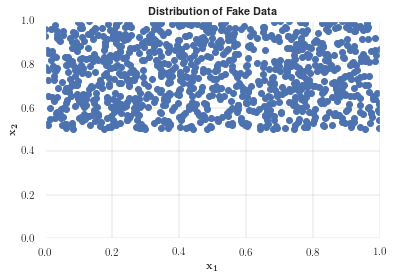
\includegraphics[width = 8cm]{Fake Uniform Distribution.png}
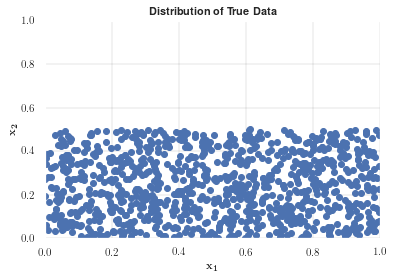
\includegraphics[width = 8cm]{True Uniform Distribution.png}
\caption{Distribution of true and fake data}
    \label{fig:uniform_distri}
\end{figure}
\subsection{Fix Generator; Train the Discriminator}
\label{sec: 1}
We first fix the generator and train the discriminator and after the training, we will try visualizing the process by feeding the discriminator points from both true and the fake distribution. The generator we choose is simply the identity one, meaning $G(z) = z$. The discriminator is a resNet according to Algorithm \ref{alg:disc} with $N_d=20$ layers. We set the learning rates at $\alpha_g = 0, \alpha_d = 0.001$. We use a mini-batch stochastic gradient descent with batch size $m = 100$ and 5000 iterations. Figure \ref{fig:gen_freeze_loss} shows the loss for both the generator and discriminator.
\begin{figure}[H]
    \centering
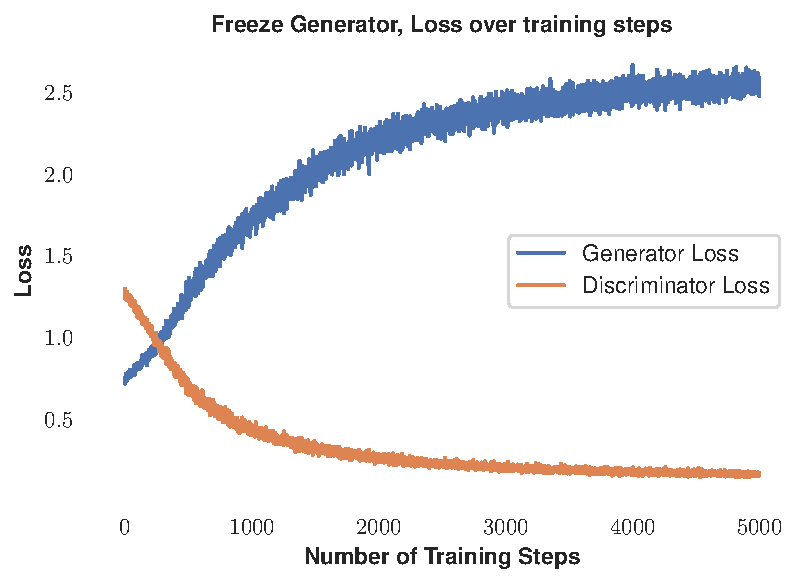
\includegraphics[width = 10cm]{Freeze_generator.pdf}
\caption{Loss over iteration}
    \label{fig:gen_freeze_loss}
\end{figure}
We observe that the discriminator loss decreases as generator loss increases, which is consistent to the fact that they are in a minimax game. The improvement of discriminator is at the cost of the higher generator loss. Although it is a simple training experiment, we can visualize the discriminator of how it discriminates data from true distribution and fake distribution through forward propagation, in other words, the evolution of points. Figure \ref{fig:evo_1} shows the evolution of true/fake data points in the process of the discriminator. The same plot also shows whether the capacity of the discriminator resNet is enough. Note that in the forward propagation algorithm, the maximum change in each coordinate of input $x$ is $\pm 0.1$ because the layer is activated by  $\tanh(x)\in (-1,1)$. Therefore in the two dimensional case with a 20-layer resNet, the maximum distance $x$ can move is $2\sqrt{2}$. We will see if the points can be moved in the correct regions within such distance.
\begin{figure}[H]
    \centering
    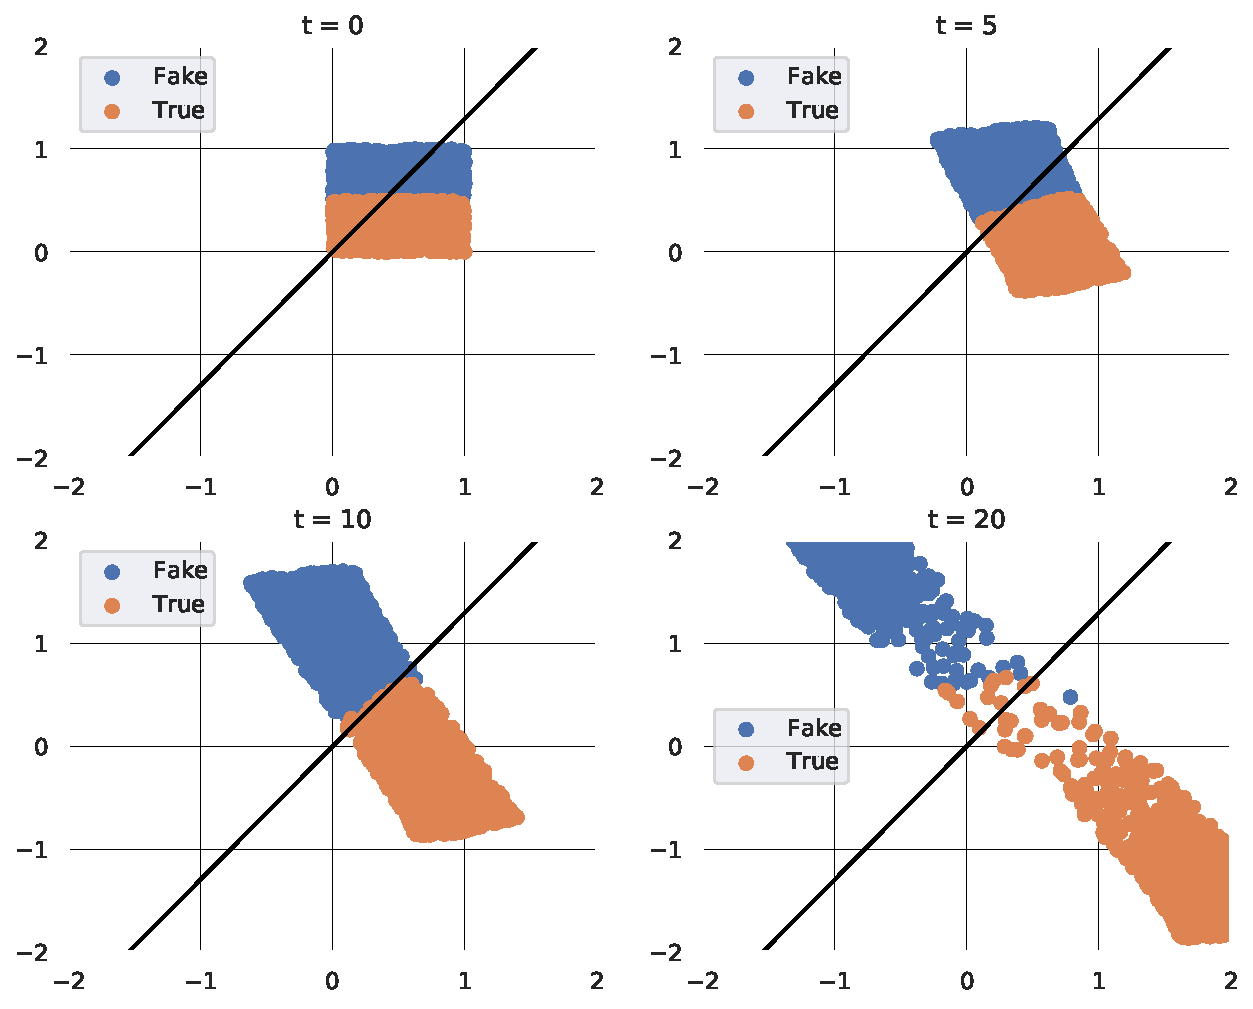
\includegraphics[width = 13cm]{Evo_1.pdf}
    \caption{Evolution of Points through Discriminator}
    \label{fig:evo_1}
\end{figure}
The black line is defined as $w^Tx +b =0$ according to the Algorithm \ref{alg:disc}, which is the decision boundary fixed by the last layer of the discriminator. We can see that as the process goes on, points are moved further away from the line accordingly. It shows how the control "drags" the points to their corresponding regions in order to minimize the terminal cost. Since moving distance of the points to the corresponding region is much less than $20\sqrt{2}$, we can determine that the discriminator resNet has enough capacity in this case.

\subsection{Fix Discriminator; Train Generator}
\label{sec: 2}
We now fix the discriminator with decision boundary $x_2 = 0.5$, meaning that points with $x_2 < 0.5$ will be classified as points from true distribution. We build the generator according to Algorithm \ref{alg:gen} with $N_g = 20$. We will use a learning rate $\alpha_g = 0.001, \alpha_d = 0$ and a mini-batch stochastic gradient descent with batch size $m = 100$ and 5000 iterations.
Figure \ref{fig:freeze_disc}, \ref{fig:distri_disc} shows the loss over the iteration steps and evolution of points under the control of generator.
\begin{figure}[H]
    \centering
    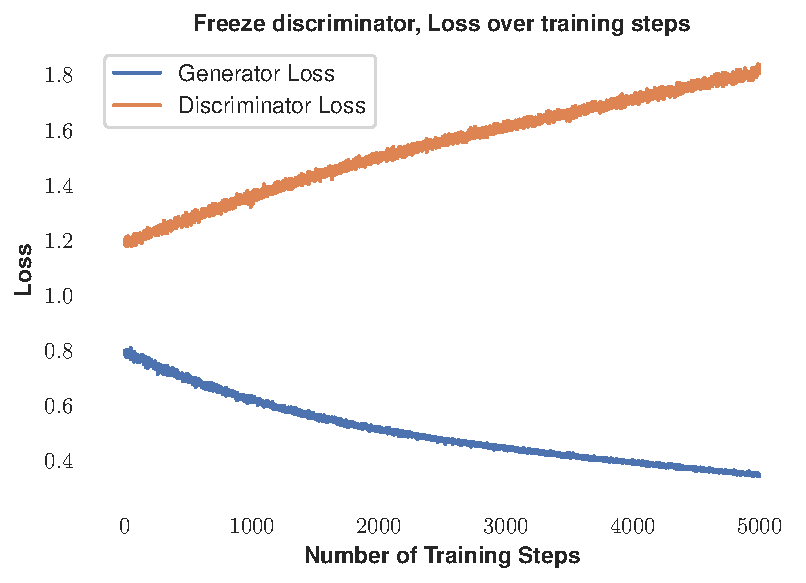
\includegraphics[width= 10cm]{Freeze_discriminater.pdf}
    \caption{Loss over iteration}
    \label{fig:freeze_disc}
\end{figure}
\begin{figure}[H]
    \centering
    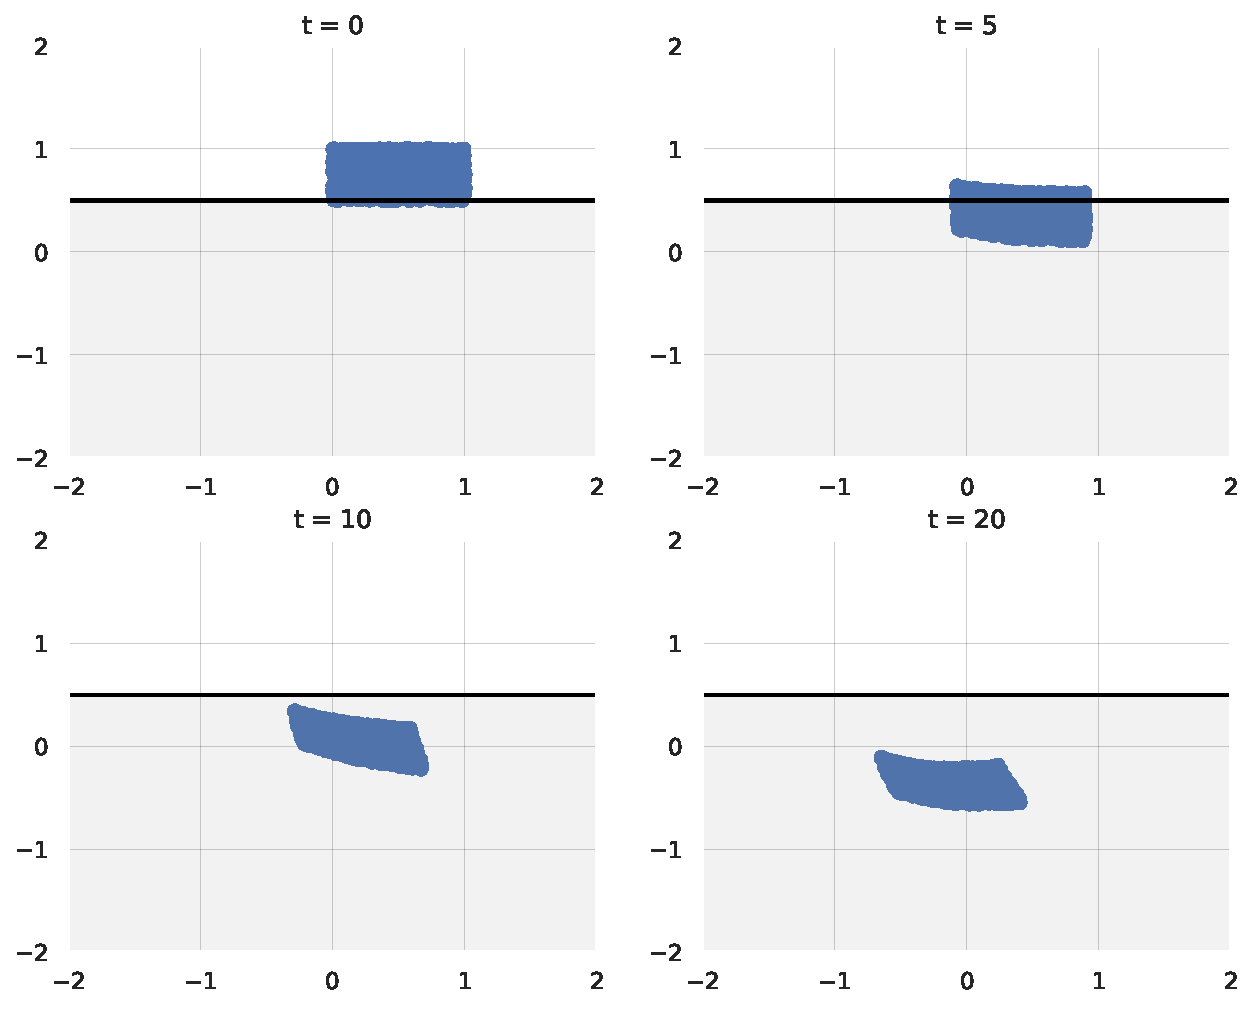
\includegraphics[width = 13cm]{Evo_2.pdf}
    \caption{Evolution of Points through Generator}
    \label{fig:distri_disc}
\end{figure}
Similarly, we can observe that the generator loss reduces at the cost of discriminator loss, illustrating the minimax game structure between the two. Moreover, in the evolution figure, the grey-shaded area is the target region and we can see the generator drags the points deeper and deeper into the target region to minimize the generator loss.
\subsection{GAN: Train the Generator and Discriminator at the same time}
Now, we have all the trivial cases done. Let's train the generator and discriminator together at the same time according to Algorithm \ref{alg:grad_d}. After training, we expect to have a good generator which can transform the noise inputs from the upper half (i.e. $[0,1] \times [0.5,1]$) to points from the true distribution, the lower half (i.e. $[0,1] \times [0,0.5]$). Moreover, in order to have a good generator, we must have a good discriminator beforehand to learn the rules of the true distribution and hence, "guide" the generator. In the experiment, I find the generator learns quicker than the discriminator with the learning rate pair $(\alpha_g,\alpha_d) = (0.001,0.001)$, meaning the minimax game is dominated by the generator. However, as the generator becomes too good before discriminator learns the features of true distribution, the algorithm requires more iterations to reach an equilibrium. In the following plots, I use $(\alpha_g,\alpha_d) = (0.0001,0.001)$. Additionally, comparing to trivial cases in the previous subsections, the real game dynamic between the generator and the discriminator complicates the training process and hence I use 10000 iterations. I will keep $N_g = N_d = 20$ the same as above because it has been validated that they have enough capacity. 
\begin{figure}[H]
    \centering
    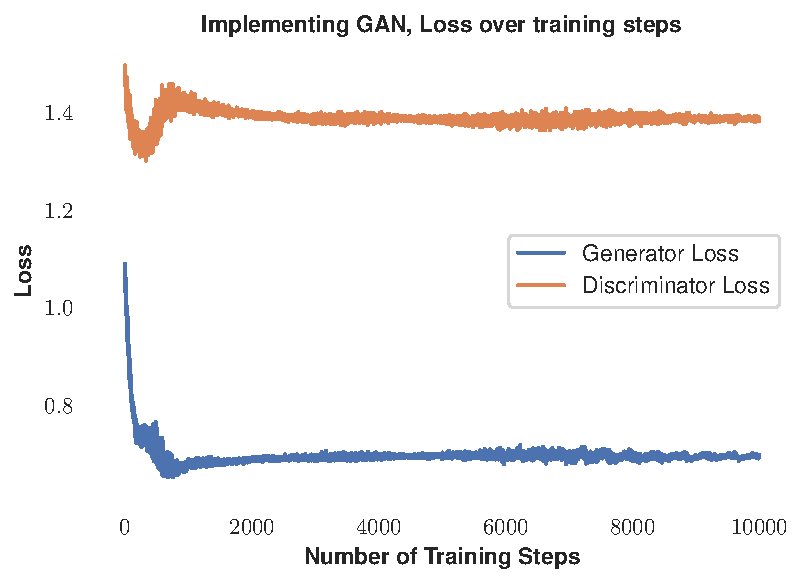
\includegraphics[width = 10cm]{GAN.pdf}
    \caption{Loss over iteration}
    \label{fig:Gan}
\end{figure}
\begin{figure}[H]
    \centering
    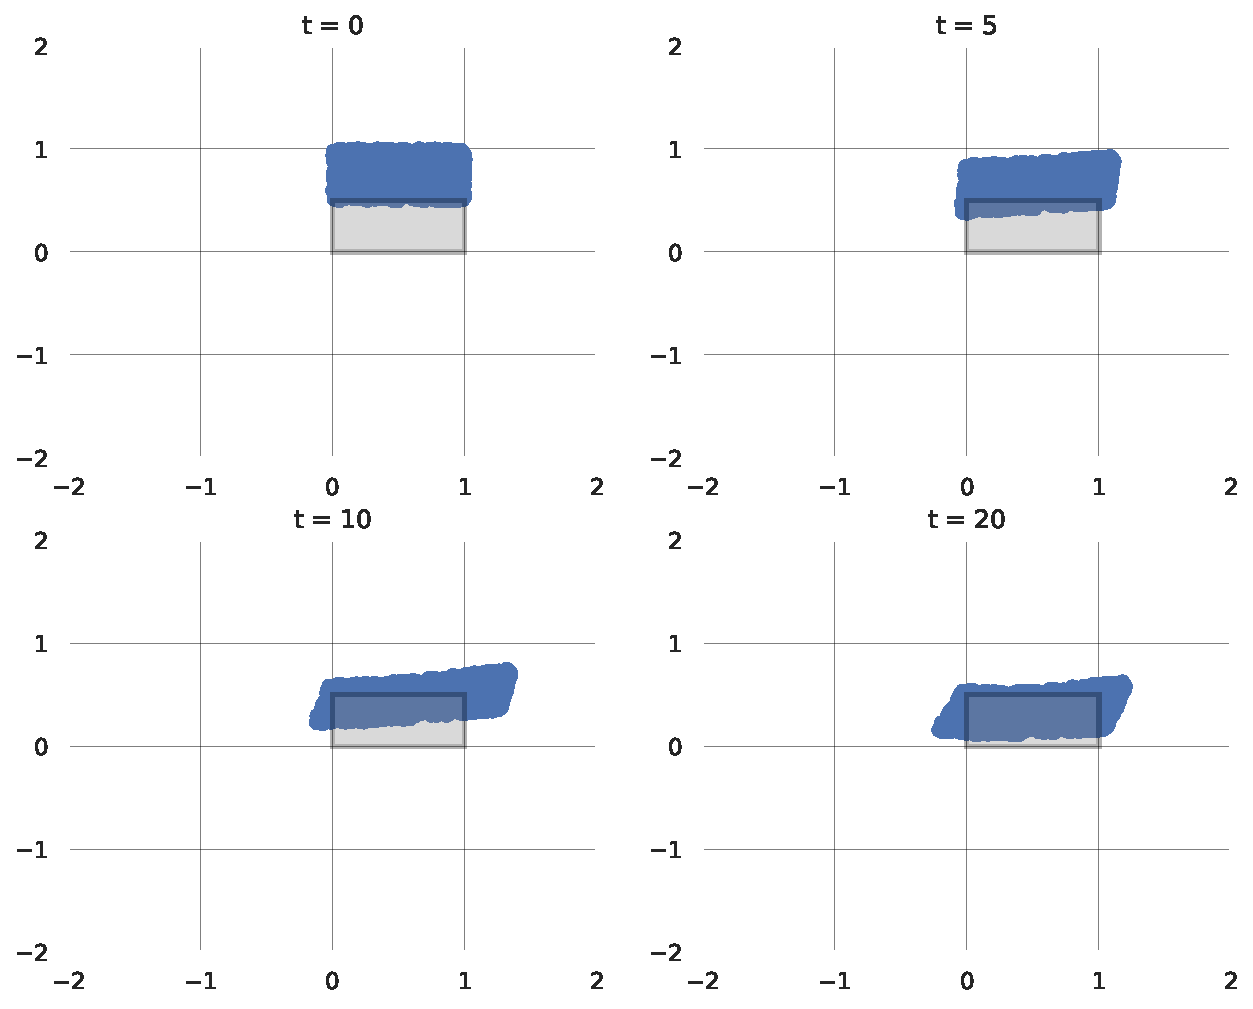
\includegraphics[width = 13cm]{Evo_3.pdf}
    \caption{Evolution of Points through Generator}
    \label{fig:GAN-gen}
\end{figure}
\begin{figure}[H]
    \centering
    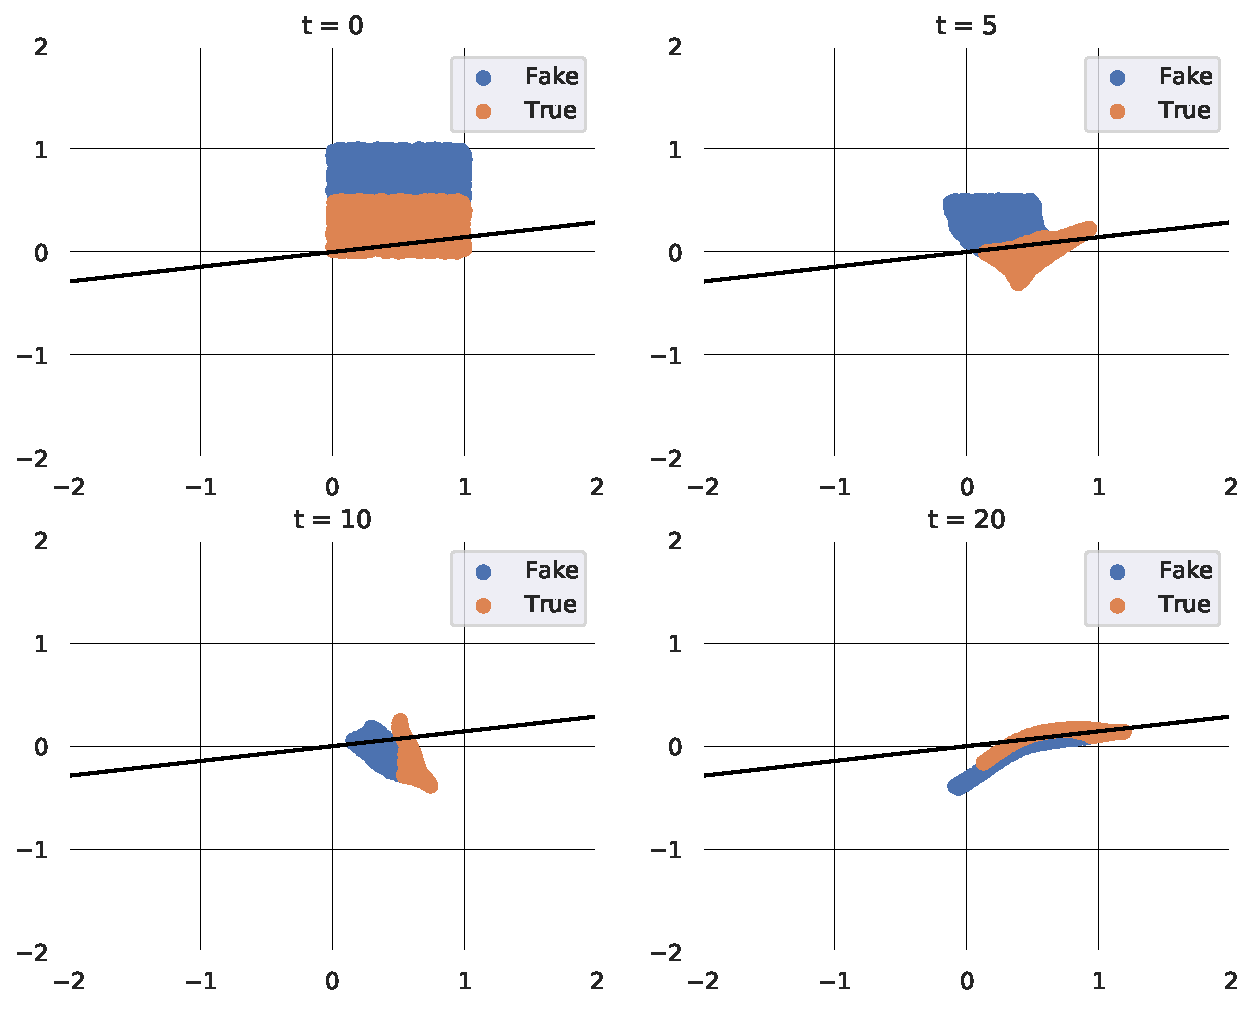
\includegraphics[width = 13cm]{Evo_4.pdf}
    \caption{Evolution of Points through Discriminator}
    \label{fig:GAN-disc}
\end{figure}
In Figure \ref{fig:GAN-gen}, the shaded area is the target region. We can see that a trained generator will move the points from the fake distribution in a way to imitate the true distribution in the end. However, we can see that some points are still out of the true distribution box. It means the generator is still not perfect after 10000 iterations and the two players have not reached a global optimality. In Figure \ref{fig:GAN-disc}, we observe that when $t = 20$, data points from both the true distribution and fake distribution clustered along the decision boundary. It illustrates that the generator is good enough to cheat the discriminator so that it is not able to decide whether the point is from the true distribution and fake distribution. Overall, we can conclude that given the discriminator, the generator is clever enough to cheat it while the discriminator has to learn more about the true distribution to guide the generator to a better result. In Figure \ref{fig:Gan}, because of the minimax game structure between the generator and the discriminator, it is difficult to visualize the improvement of the algorithm with only the plot of the loss over iterations. It is likely that the stable loss in later training steps means the algorithm is trapped in a local optimality while it can also mean both the generator and the discriminator are learning. We will provide more details in the next example.
\section{Normal Distribution Experiment}
In this section, we will conduct the same experiment on a different distribution: normal distribution. Let the true distribution be $(x_1,x_2)^T \sim \mathcal{N}\left((0,0)^T, \Sigma\right)$ and the fake distribution be $(z_1,z_2)^T \sim \mathcal{N}\left((1,1)^T, \Sigma\right)$, where $\Sigma = \begin{bmatrix}
0.05 & 0\\
0 & 0.05\\
\end{bmatrix}$. The discriminator is more difficult to train compared to the previous experiment because the data points from fake distribution and true distribution overlap. It means that even with a primitive generator (e.g. the identity), given a data point, the discriminator can not easily determine which distribution it comes from. 
\begin{figure}[H]
    \centering
    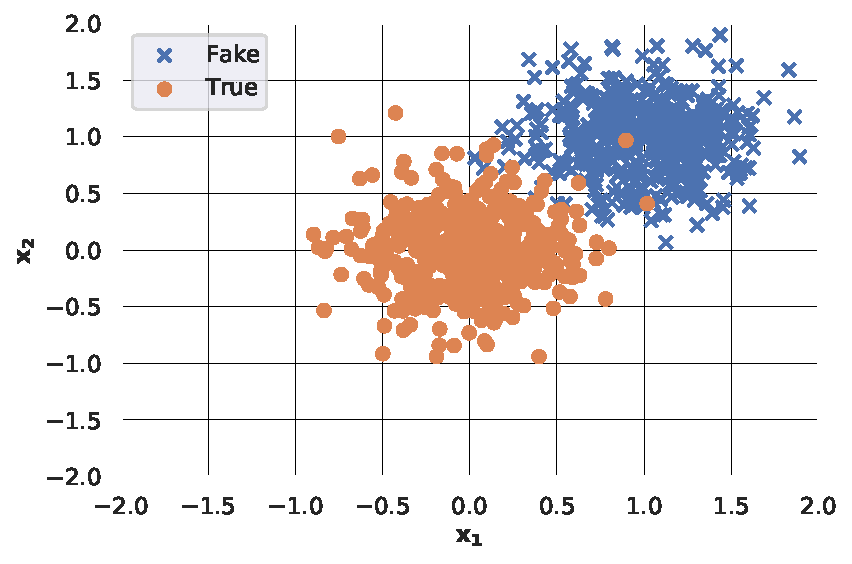
\includegraphics[width = 12cm]{Gaussian Distribution.pdf}
    \caption{Gaussian Distribution}
    \label{fig:gau}
\end{figure}
Figure \ref{fig:gau} shows samples from the true and fake distribution. In this experiment, we will omit the preliminary parts similar to section \ref{sec: 1}, \ref{sec: 2} and we directly train according to the \ref{alg:grad_d} algorithm.

As mentioned in the previous section, it is difficult to directly visualize the success of the algorithm by looking at the loss over iterations. Therefore, we will need a new measure of success. Since the true distribution is known, we will define the generated likelihood from a fixed noise input $z_1 , z_2 , ... , z_n$ as:
$$ \mathcal{L}(\theta^G) = \prod_{i = 1}^{n} f\left (G_{\theta^G}(z_i)\right), \text{   $f$ is the probability density function of true distribution}$$
In this case, 
$$ f (\boldsymbol{x}) =\frac{1}{\sqrt{(2 \pi)^{2} \cdot \det (\boldsymbol{\Sigma})}} e^{-\frac{1}{2}x^{T} 
\boldsymbol{\Sigma^{-1}} x},  \quad \Sigma \text{ is defined above}$$
We can further simplify in our case that to maximize the likelihood is equivalent to minimize the following $$l(\theta^G) = \sum_{i = 1}^{n} G(z_i)^T \Sigma^{-1} G(z_i) \propto \sum_{i = 1}^{n} ||G(z_i)||^2 ,$$
We will call this number the negative log-generated likelihood and we will use this to measure the success of the algorithm. Furthermore, to simplify, we will fix a group of test prior input noise points at the beginning and compute the number based on the points generated by those points. Ideally, we will see this number decrease which indicates that the probability that such group of generated points are sampled from the true distribution increases, meaning the generator is improving. Due to the computational cost, we will take $n= 10$ samples from noise input and compute the log-generated likelihood.
We apply the same logic to deduce the capacity of the generator: We find that in this case the distance points from fake distribution have to travel is $(1,1) \rightarrow (0,0) = \sqrt{2}$ and we a 20-layered resNet has the maximum capacity to move points for a distance of $2\sqrt{2}$. Hence the capacity of $N_g = 20$ is reasonable. Similar to the case in uniform distribution, when training the GAN, we implement the learning rate $\alpha_g = 0.0001, \alpha_d = 0.001$ to avoid the dominance of the generator. We will set $N_d = 20$ and run the iterative algorithm \ref{alg:grad_d} for 10000 times.
We can see from Figure \ref{fig:gauiter} that during the first 2000 iterations, the generator loss and discriminator loss changes significantly and accordingly, the log generated likelihood decreases. It means that our algorithm is working. Moreover, we observe that the discriminator loss decreases at the beginning at the cost of the generator loss. We prefer this structure instead of the other way around because without an accurate discriminator, the generator will definitely fail in imitating the true distribution. Also, it validates that our learning rate pair is wisely chosen. After about 2000 iterations, we find the losses are relatively stable and the log generated likelihood remains almost the same. It suggests that after 2000 training steps, the algorithm ceases to learn and is close to a local optimality. Figure \ref{fig:comparison} shows the result of generated distribution. We can see that the generated distribution and true distribution are very similar.
Figure \ref{fig:evo_dis_gau} shows how points from two distributions evolves under the control of the discriminator. It is worth noting that in this case, the discriminator outputs all the points centered along the decision boundary, indicating that the generator is well trained. Figure \ref{fig:evo_gen_gau} shows how points from noise prior distribution evolve under the control of the discriminator. 
\begin{figure}
    \centering
    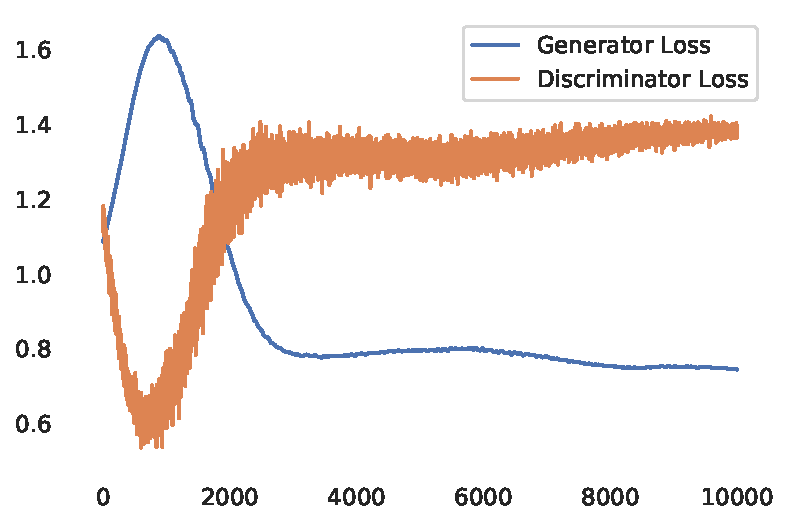
\includegraphics[width = 8cm]{GAN_gau.pdf}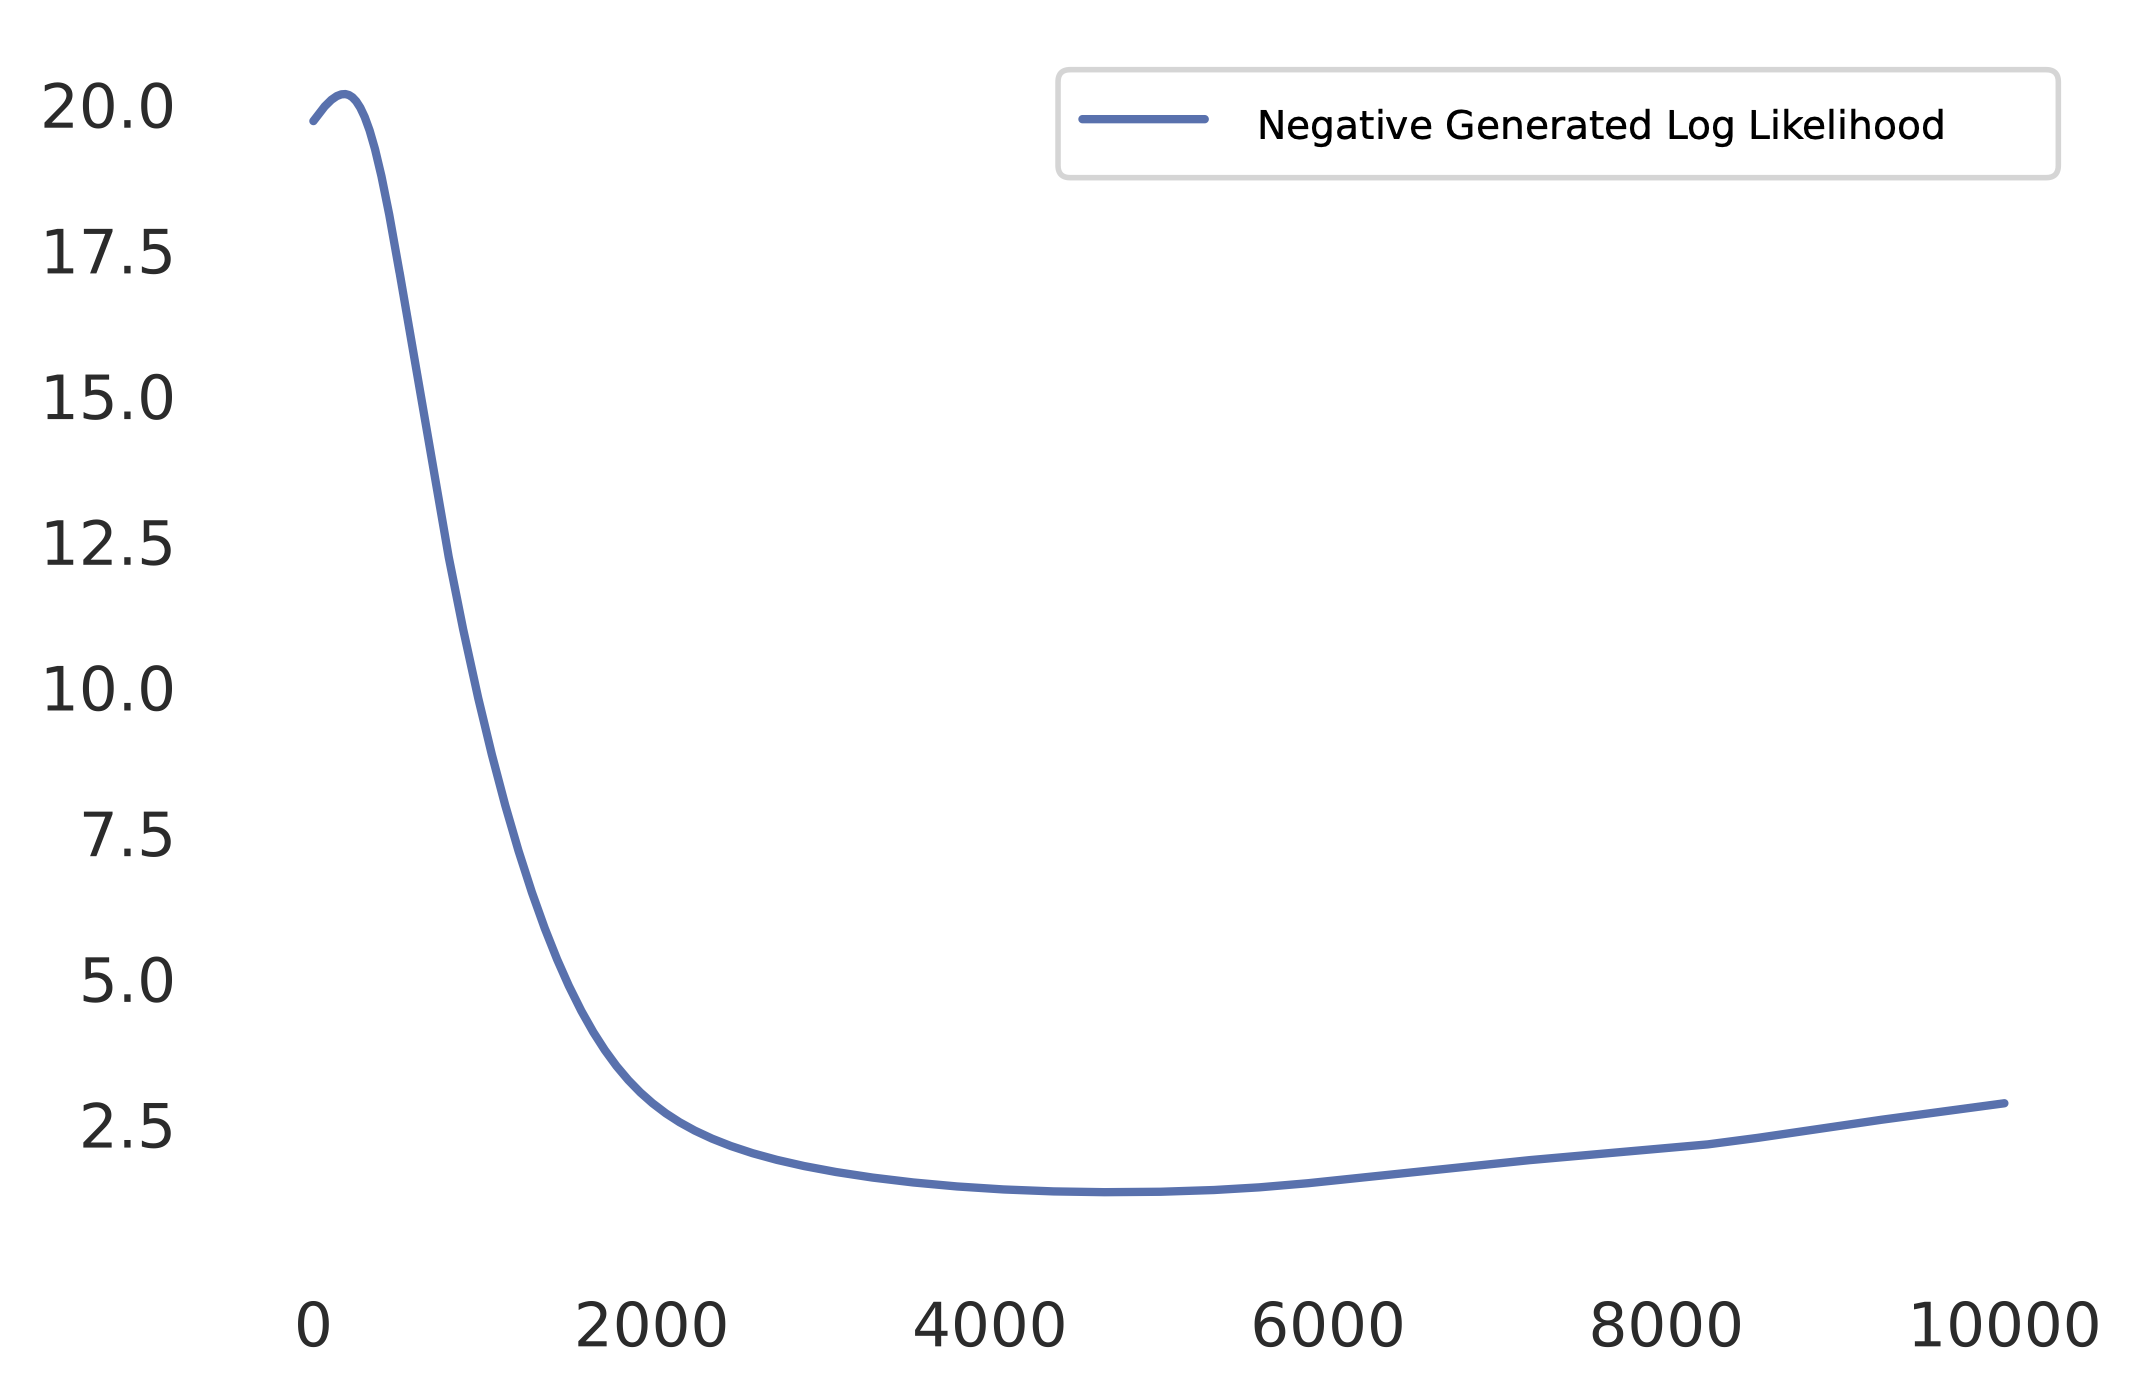
\includegraphics[width = 8cm]{GAN_gau_likeli.png}
    \caption{Loss, negative log-generated likelihood over iteration}
    \label{fig:gauiter}
\end{figure}
\begin{figure}
    \centering
    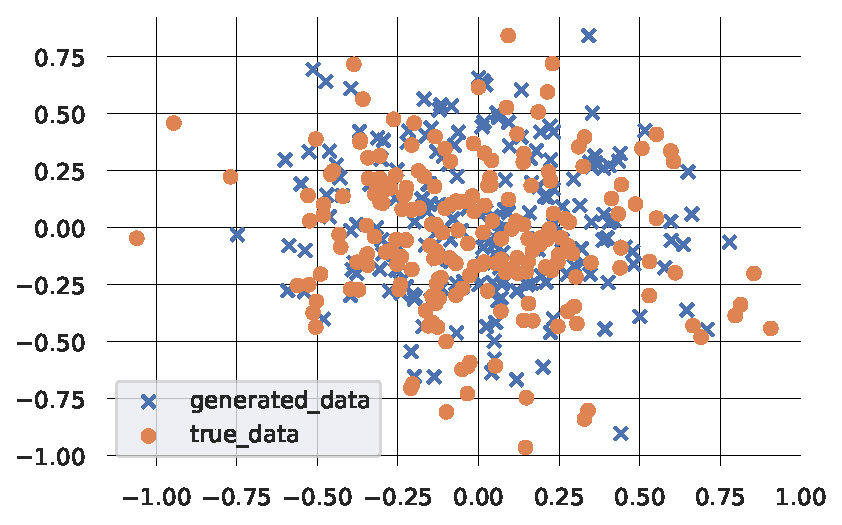
\includegraphics[width = 13cm]{comparison.pdf}
    \caption{Generated Data vs. True Data}
    \label{fig:comparison}
\end{figure}
\begin{figure}
    \centering
    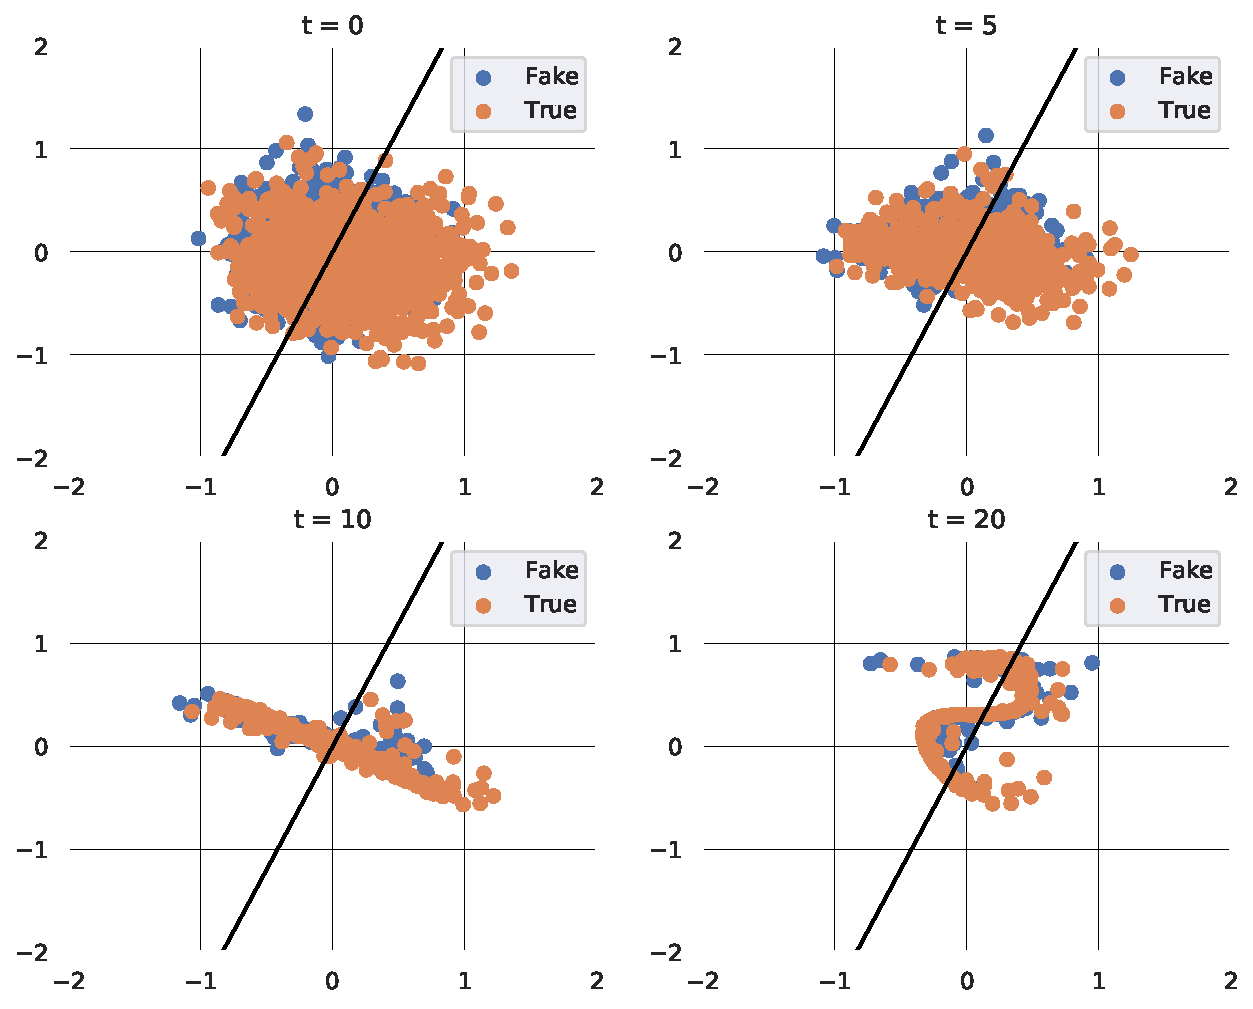
\includegraphics[width = 13 cm]{Evo_5.pdf}
    \caption{Evolution of Points through Discriminator}
    \label{fig:evo_dis_gau}
\end{figure}
\begin{figure}
    \centering
    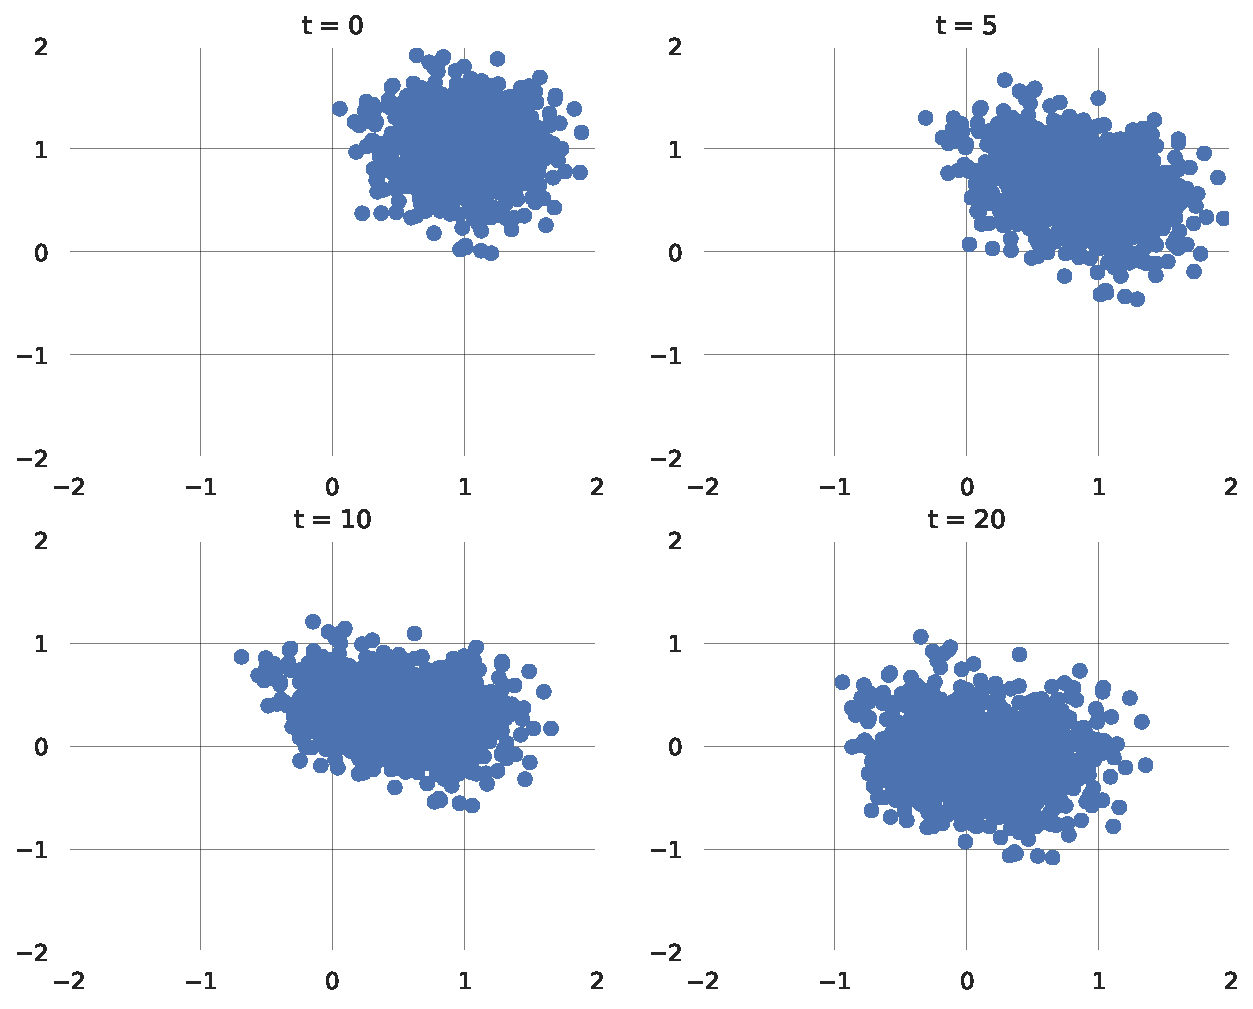
\includegraphics[width = 13 cm]{Evo_6.pdf}
    \caption{Evolution of Points through Generator}
    \label{fig:evo_gen_gau}
\end{figure}



\chapter{Conclusion and Discussions}
\label{chp-conclusion}
\section{Conclusion}
In this paper, we introduce a mathematical formulation of the GAN algorithm in terms of the mean field optimal control theory. Moreover, experiments on imitation of normal distribution and uniform distribution are done to provide empirical understanding on the training strategy. Lastly, the evolution of points under the control of both the discriminator and the generator is visualized to understand the resNet from the perspective of dynamical systems.

\section{Discussion}
As the GAN algorithm is theoretically formulated in the paper in terms of mean field optimal control, we can further apply important results from the optimal control theory like HJB equation and Pontrygin maximum principle to further analyze the problem theoretically. Moreover, as the minimax game structure is embedded in the GAN algorithm, it may be possible to find a relationship between optimal control and the Nash Equilibrium. In the experiments, the results on simple distributions are encouraging and we only experiment on the same family of distribution for both fake and true data distribution. It will be interesting to visualize how generator controls a uniform distribution to imitate a normal distribution. More experiments and visualizations on more complicated distributions may be insightful in the problem. 


%% If your thesis has different "Parts", use commands such as the following:
%\part{First Part\label{part:one}}%
% \input{chap1}
%\input{chap2} % further chapters -- change file names to meaningful things...
%\input{chap3}
%\part{Second Part\label{part:two}}%
%\input{chap4}
%\input{chap5}
%\input{chap6}


%%%%% Appendices start %%%%%%%%%%%%%%%%
%% Comment out the following if your thesis has no appendix

% \appendix

% \chapter{Appendix}

% % \input{appendix}
% \lipsum

%% Note: If your thesis has more than one appendix, NYU requires a "list of
%% appendices" page before the body of the thesis. I don't provide the tools
%% to create that here, so you're on your own for that one... Sorry.


%%%% Input bibliography file %%%%%%%%%%%%%%%
%% For computer science dissertations, I'd recommend using the bibly package
%% to automatically create the .bib file from your citations:
%% https://github.com/michael-emmi/bibly

\cleardoublepage
\phantomsection
\bibliographystyle{ieeetr}
\addcontentsline{toc}{chapter}{Bibliography}
\bibliography{refs} % Entries are in the refs.bib file

% The following is just for the sample template,
% I'd recommend deleting this and using the \bibliography command above
% \begin{thebibliography}{99}
% \bibitem[Lamport, 1994]{lamport94}
%   Leslie Lamport,
%   \textit{\LaTeX: a document preparation system},
%   Addison Wesley, Massachusetts,
%   2nd edition,
%   1994.
% \end{thebibliography}


\end{document}

%%% Local Variables:
%%% mode: latex
%%% TeX-master: t
%%% End:
